\documentclass[8pt,compress]{beamer}
\usepackage{multicol}
\usepackage{graphics}
%\usepackage{cascadia-code}
\usepackage{listings}
\usepackage{soul}
\usepackage[default]{sourcesanspro}
\usepackage[T1]{fontenc}
\usepackage[font=tiny]{caption}
%\renewcommand*\familydefault{\ttdefault} %% Only if the base font of the document is to be typewriter style
\newcommand\LightBold[1]{\textcolor{VSBlueLight}{\textbf{#1}}}
\newcommand\DarkBold[1]{\textcolor{VSBlueDark}{\textbf{#1}}}
\newcommand\DarkBoldP[1]{\textcolor{VSPurpleDark}{\textbf{#1}}}
\usepackage[T1]{fontenc}

\usetheme{Dark}


% Title Slide
\title{Claims Investigation Committee Multi-Testing Input Device}
\subtitle{ECE-4820: Electrical and Computer Engineering Design II}
\author[Garza, Baker, Sah]{Dylan-Matthew Garza \and Daniel Baker \and Rohullah Sah \and}

\institute[VFU] % (optional)
{
      Department of Electrical and Computer Engineering\\
      Western Michigan University
      \and
      ZF Group\\
      Auburn Hills, MI
}
\date{Fall 2024}
\titlegraphic{
\includegraphics[height=2cm]{assets/WMU_Logo.png}\hspace{1cm}
\includegraphics[height=2cm]{assets/zf.png}}



\begin{document}
%==============================================================================
% Introduction slide
%==============================================================================
\begin{frame}[plain]
  \titlepage
  \small
  \begin{multicols}{2}
      Faculty Advisor:\\
      Dr. Janos Grantner\hfill\\
    \hfill{}\makebox[0pt][r]{Sponsor Manager}:\\
    \hfill Patrick McNally
  \end{multicols}
\end{frame}

\AtBeginSection[]
{
  \begin{frame}
    \frametitle{Table of Contents}
    \tableofcontents[currentsection]
  \end{frame}
}
\section{Introduction}
%==============================================================================
% INTRODUCTION SECTION
%==============================================================================
\subsection{ZF}
\begin{frame}
  \frametitle{ZF}
  \begin{minipage}{0.45\textwidth}
    \begin{block}{What is ZF?}
      \begin{itemize}
          \small {
            \item Global technology company and Tier 1 automotive supplier
            \item Provides advanced safety systems and vehicle control solutions
            \item Partners with major OEMs: Daimler, Chrysler, Tesla, Waymo(Google), etc.
            \item A leading innovator in commercial vehicle technology
          }
      \end{itemize}
    \end{block}
  \end{minipage}
  \hfill
  \begin{minipage}{0.45\textwidth}
    \begin{figure}
      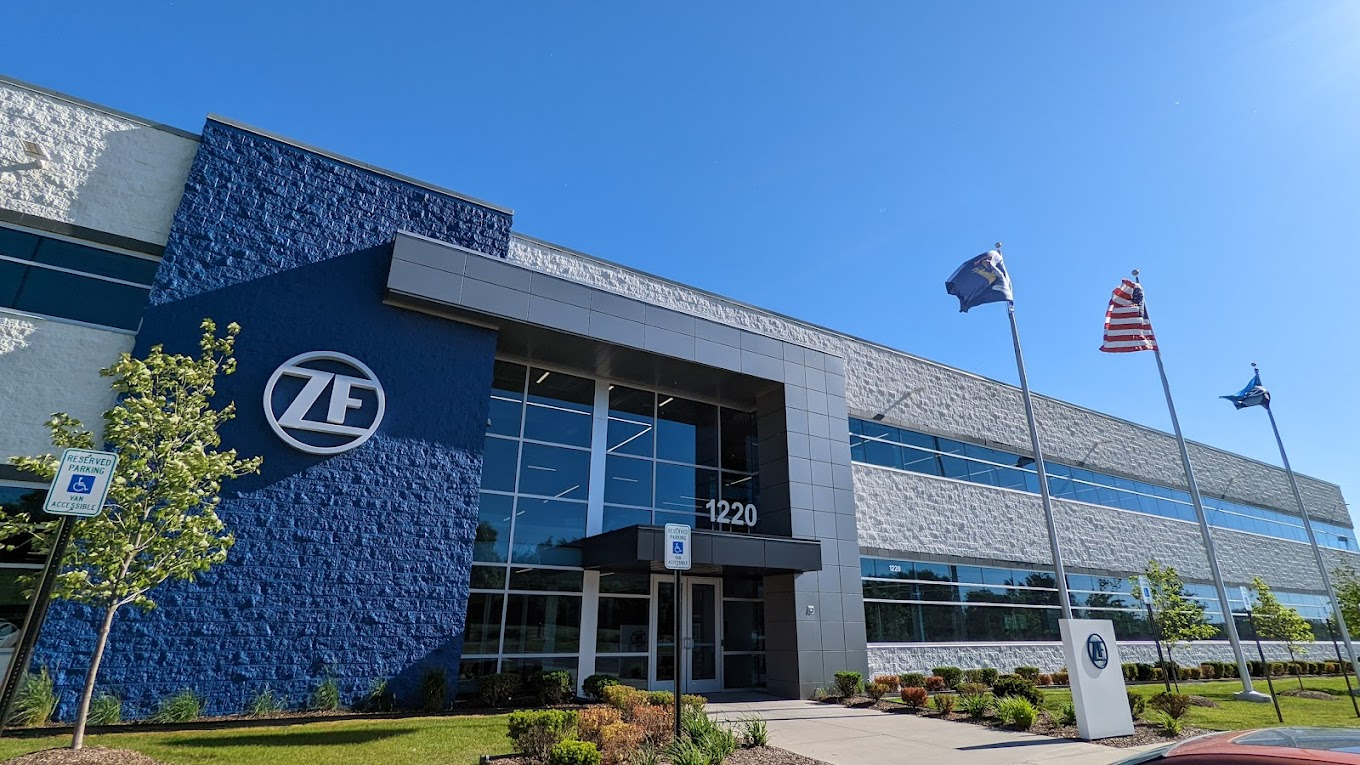
\includegraphics[width=\textwidth]{assets/misc/zf-office.jpg}
      \caption{Source: \href{google.com}{google.com}\hspace{\textwidth}
      \textit{ZF Group Office in Auburn Hills, MI}}
    \end{figure}
  \end{minipage}
  \begin{block}{Project Background}
    \begin{itemize}
        \item Claims Investigation Committee (CIC) required enhanced testing capabilities
        \item Focus on key component: Brake Signal Transmitter (BST)
        \item BST critical for highest volume commercial vehicle platform in North America (Daimler)
        \begin{itemize}
            \item Daimler Truck AG - World's largest commercial vehicle manufacturer
            \item Previous parent company of Mercedez Benz before splitting in 2021
        \end{itemize}
        \item Need for rapid, accurate analysis of field returns
    \end{itemize}
  \end{block}
\end{frame}


\subsection{Need for Multi-Testing Input Device}
\begin{frame}
    \frametitle{Need for Multi-Testing Input Device}
    \begin{block}{Project Drivers}
        \begin{itemize}
            \item Brake Signal Transmitter implementation in Daimler's new platform drive urgent need
            \item Current testing methods are too time-consuming for production volumes
            \item Need for quick validation of warranty claims
            \item Opportunity to expand test capabilities to other electronic components
        \end{itemize}
    \end{block}
    %\begin{block}{Key Components Under Test}
    \begin{block}{Key Devices Under Test (DUTs)}
    \begin{enumerate}
        \item {\DarkBold{Brake Signal Transmitter (BST)}}
        \begin{itemize}
            \item Primary focus - critical new component for 2025 production
            \item Acts as the brain that reads how hard a driver presses the brake.
        \end{itemize}
        \item {\DarkBold{Continuous Wear Sensor (CWS)}}
        \begin{itemize}
            \item Works like a monitor for your brake pads and discs
            \item Warns when brakes are wearing down using voltage
        \end{itemize}
        \item {\DarkBold{Pressure Sensor}}
        \begin{itemize}
            \item Continuously measures relative pressure in vehicle control systems
        \end{itemize}
        \item {\DarkBold{Electronic Stability Control Module (ESCM)}}
            \begin{itemize}
                \item Acts as a safety system that helps prevent skidding and rollovers
                \item Monitors the vehicle's movement and intervenes to keep it stable
            \end{itemize}
    \end{enumerate}
  \end{block}
\end{frame}

%==============================================================================
% DESIGN AND IMPLEMENTATION SECTION: Project Specifications and Overview
%==============================================================================

\section{Design and Implementation}
\subsection{Project Specifications and Overview}

\begin{frame}
  \frametitle{Project Specifications}
  \includegraphics[width=0.75\textwidth]{assets/diagrams/hardware.png}
  \begin{block}{What this project aims to accomplish:}
    \begin{enumerate}
      \item {\DarkBold{Device Interfacing}}
        \begin{enumerate}
          \item Properly read Device Signals using the ARM Cortex-M4 on the onboard microcontroller on the 
            \LightBold{STM32MP157F-DK2}:
            \begin{itemize}
              \item PWM Duty Cycle
              \item Frequency
              \item Voltages through an analog-to-digital converter (ADC)
              \item CAN frames
            \end{itemize}
        \end{enumerate}
    \end{enumerate}
  \end{block}
\end{frame}

\begin{frame}
  \frametitle{Project Specifications (cont.)}
  \large
  \begin{block}{Project Specifications}
    \large
    \begin{enumerate}
        \setcounter{enumi}{1}
      \item \DarkBold{Physical Components and Hardware}
        \begin{enumerate}
          \large
          \item Printed Circuit Board (PCB) for interfacing with DUT
          \item PCB for scaling and managing power for the DUT and to the microcontroller
          \item Enclosure for PCBs and \LightBold{STM32MP157F-DK2} board
        \end{enumerate}
    \end{enumerate}
  \end{block}
\end{frame}

\begin{frame}
  \frametitle{Project Specifications (cont.)}
  \begin{block}{What this project aims to accomplish:}
    \begin{enumerate}
        \setcounter{enumi}{2}
        \large
      \item \DarkBold{Software}
        \begin{enumerate}
            \large
          \item Custom embedded \textbf{Linux} distribution that will run on the onboard ARM Cortex-A7
            microprocessor on the \LightBold{STM32MP157F-DK2}
          \item Simple user interface web-based application
          \item Custom Webserver to process information from web application to microcontroller
          \item Communicate collected information from ARM Cortex-M4 to ARM Cortex-A7
          \item Ability to download measured data, formatted as a CSV, through the web application 
        \end{enumerate}
    \end{enumerate}
  \end{block}
\end{frame}

\begin{frame}
  \frametitle{Comprehensive System Block Diagram}
  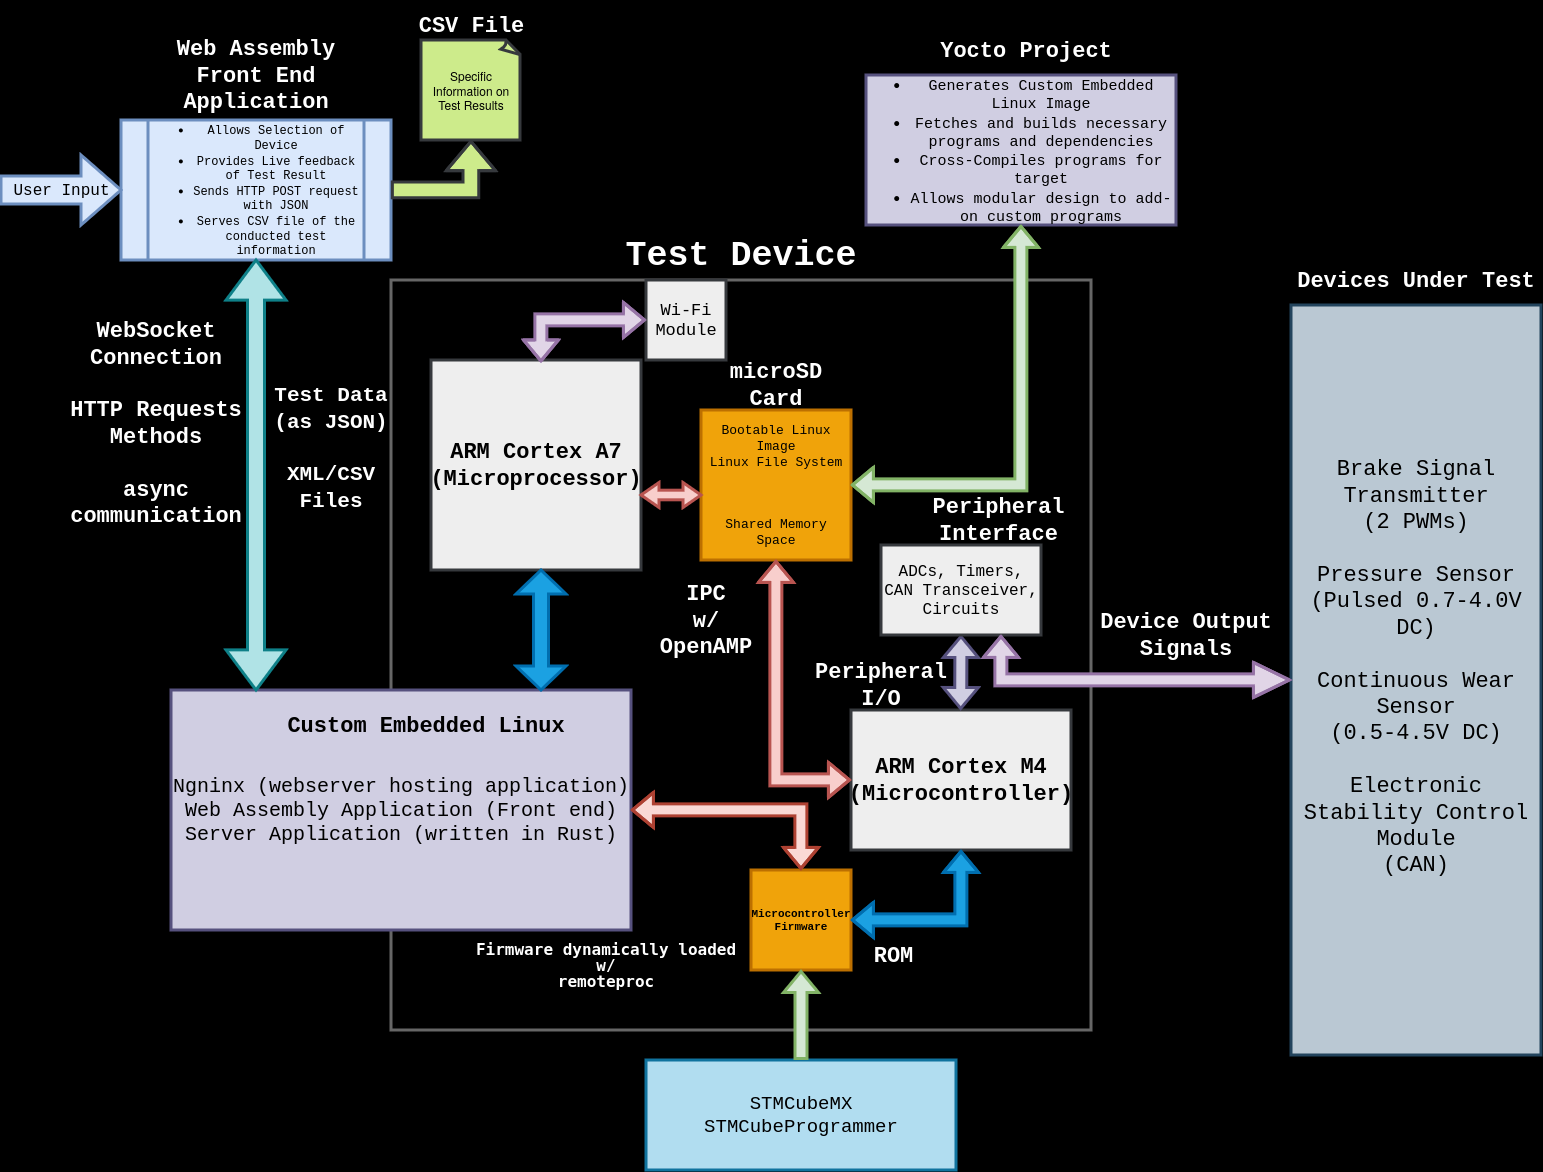
\includegraphics[width=0.90\textwidth]{assets/diagrams/block_diagram.drawio.png}
\end{frame}

%==============================================================================
% DESIGN AND IMPLEMENTATION SECTION: Gantt Chart
%==============================================================================
\begin{frame}
  \frametitle{Gantt Chart}
  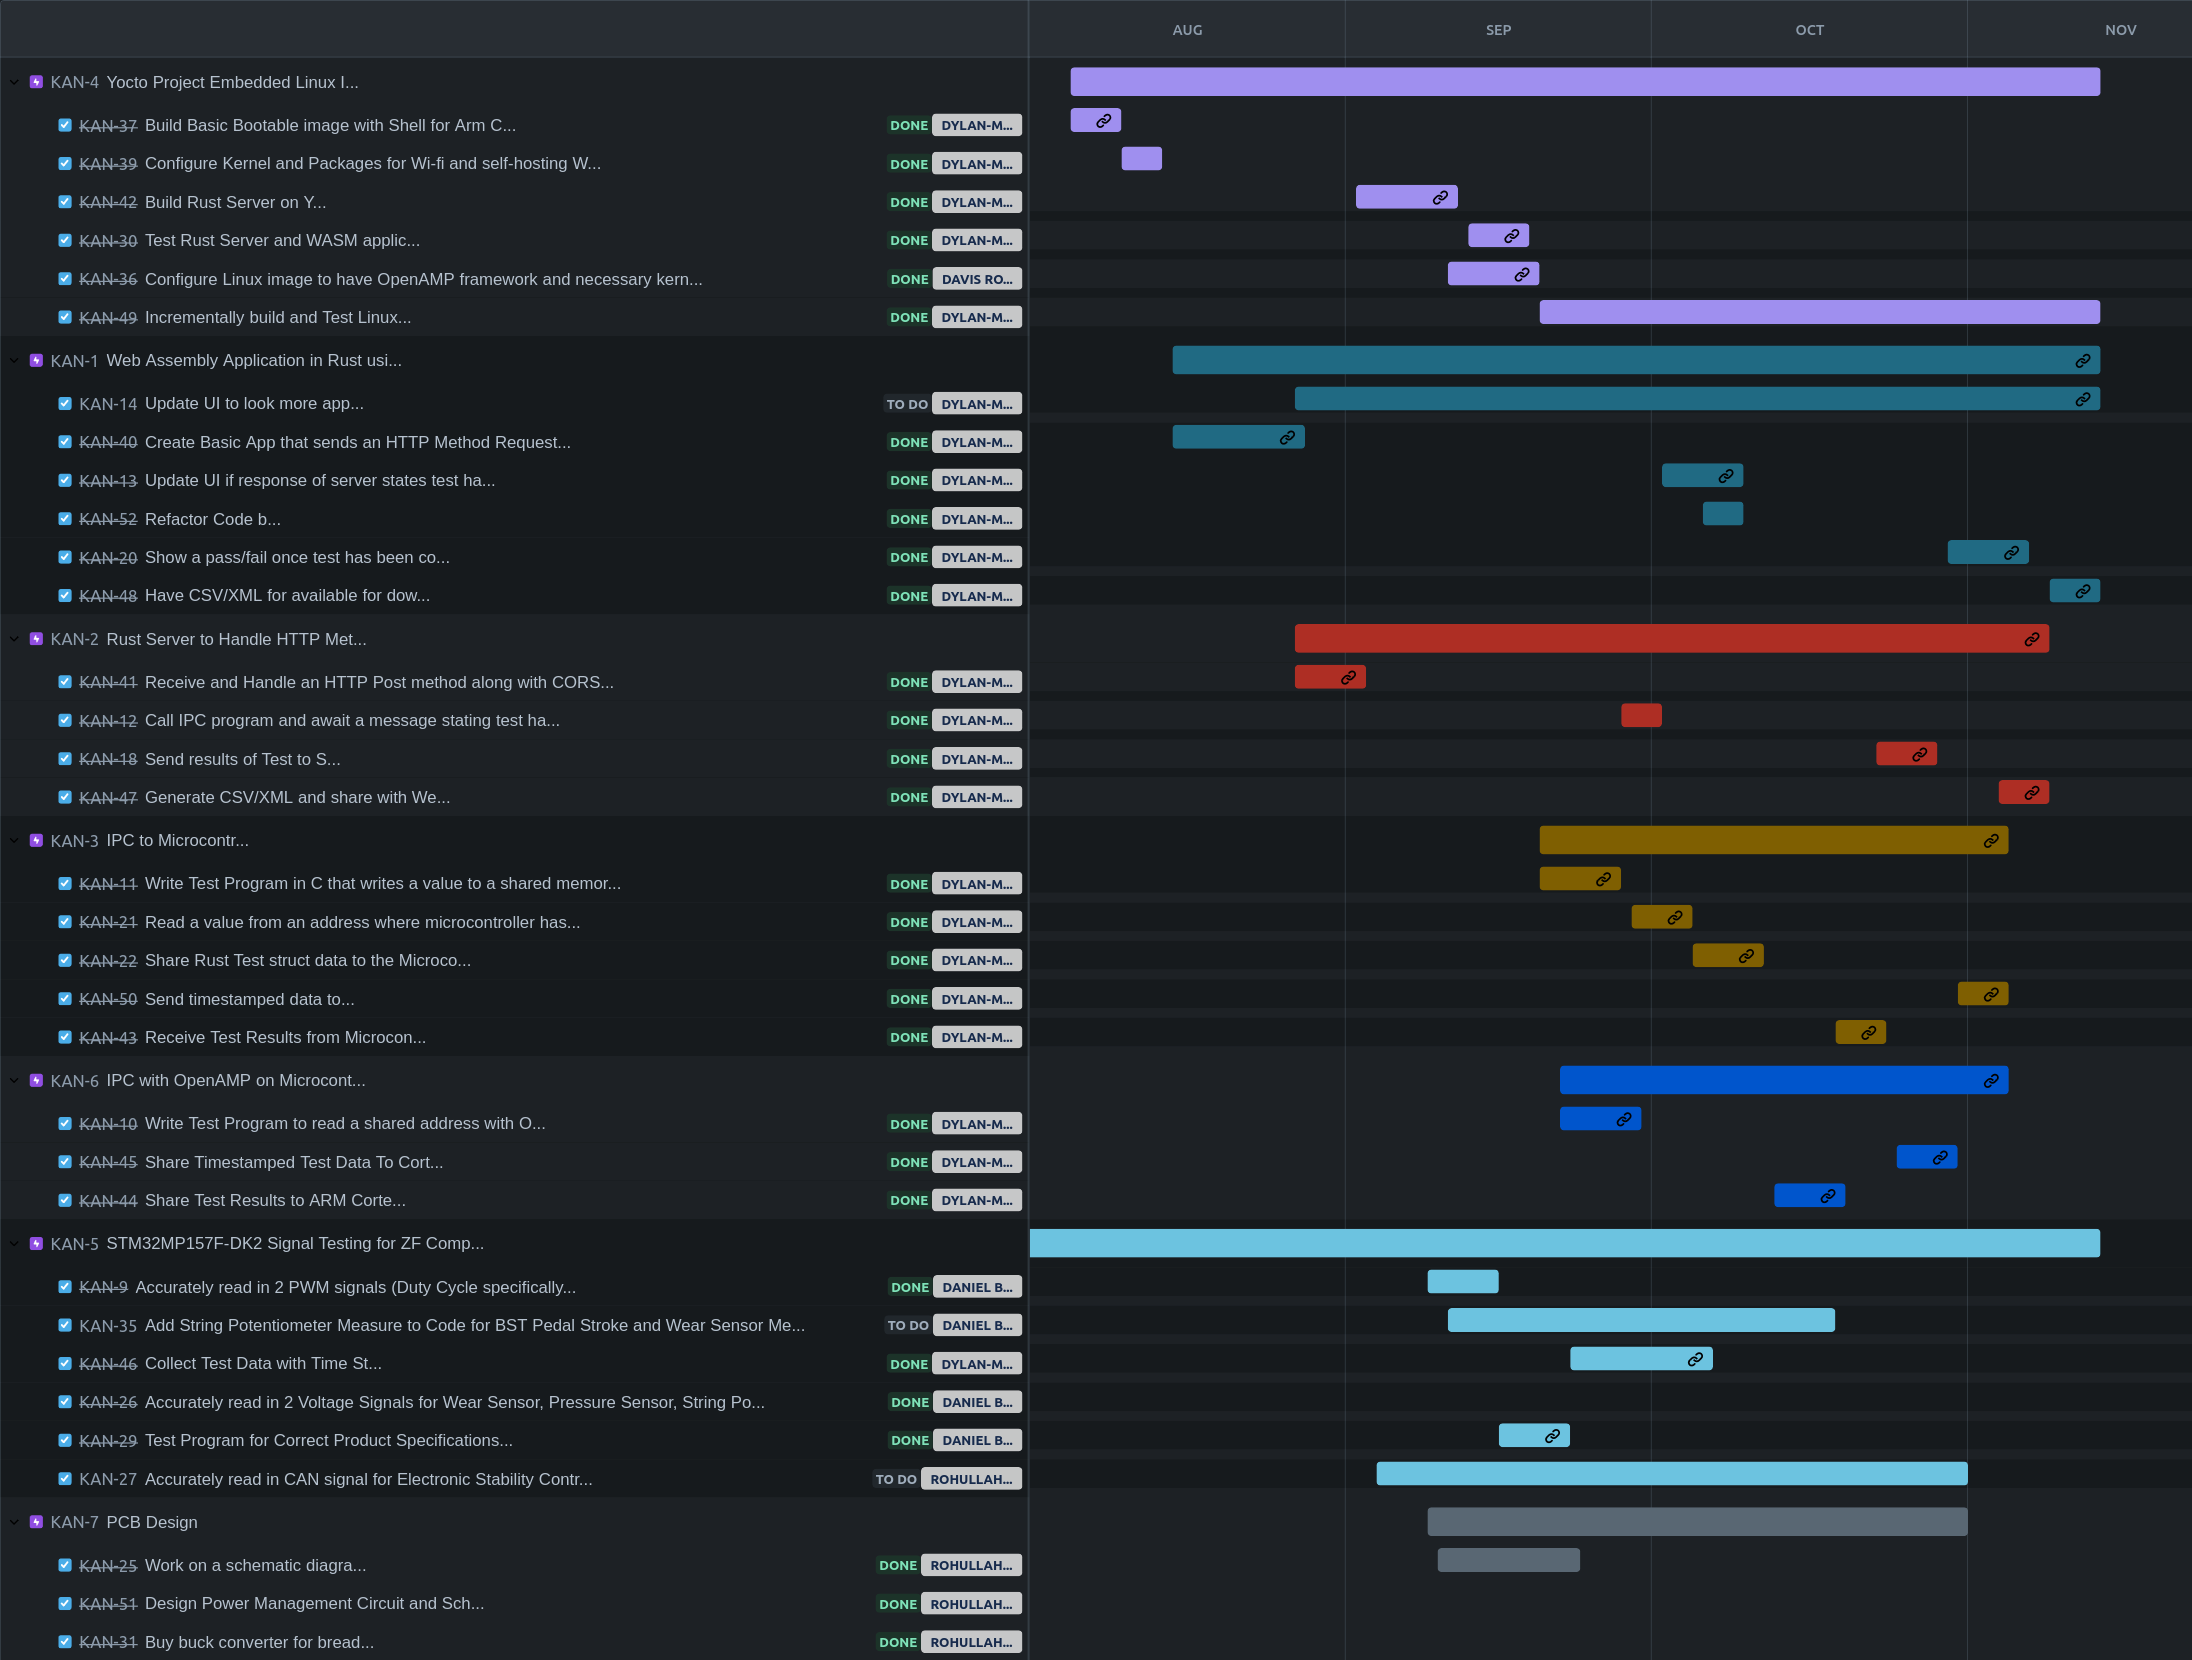
\includegraphics[width=0.875\textwidth]{assets/diagrams/gantt.png}
\end{frame}
%==============================================================================
% DESIGN AND IMPLEMENTATION SECTION: Budget Projection
%==============================================================================
\begin{frame}
  \frametitle{Budget Projection}
  \vspace{-.2025cm}
  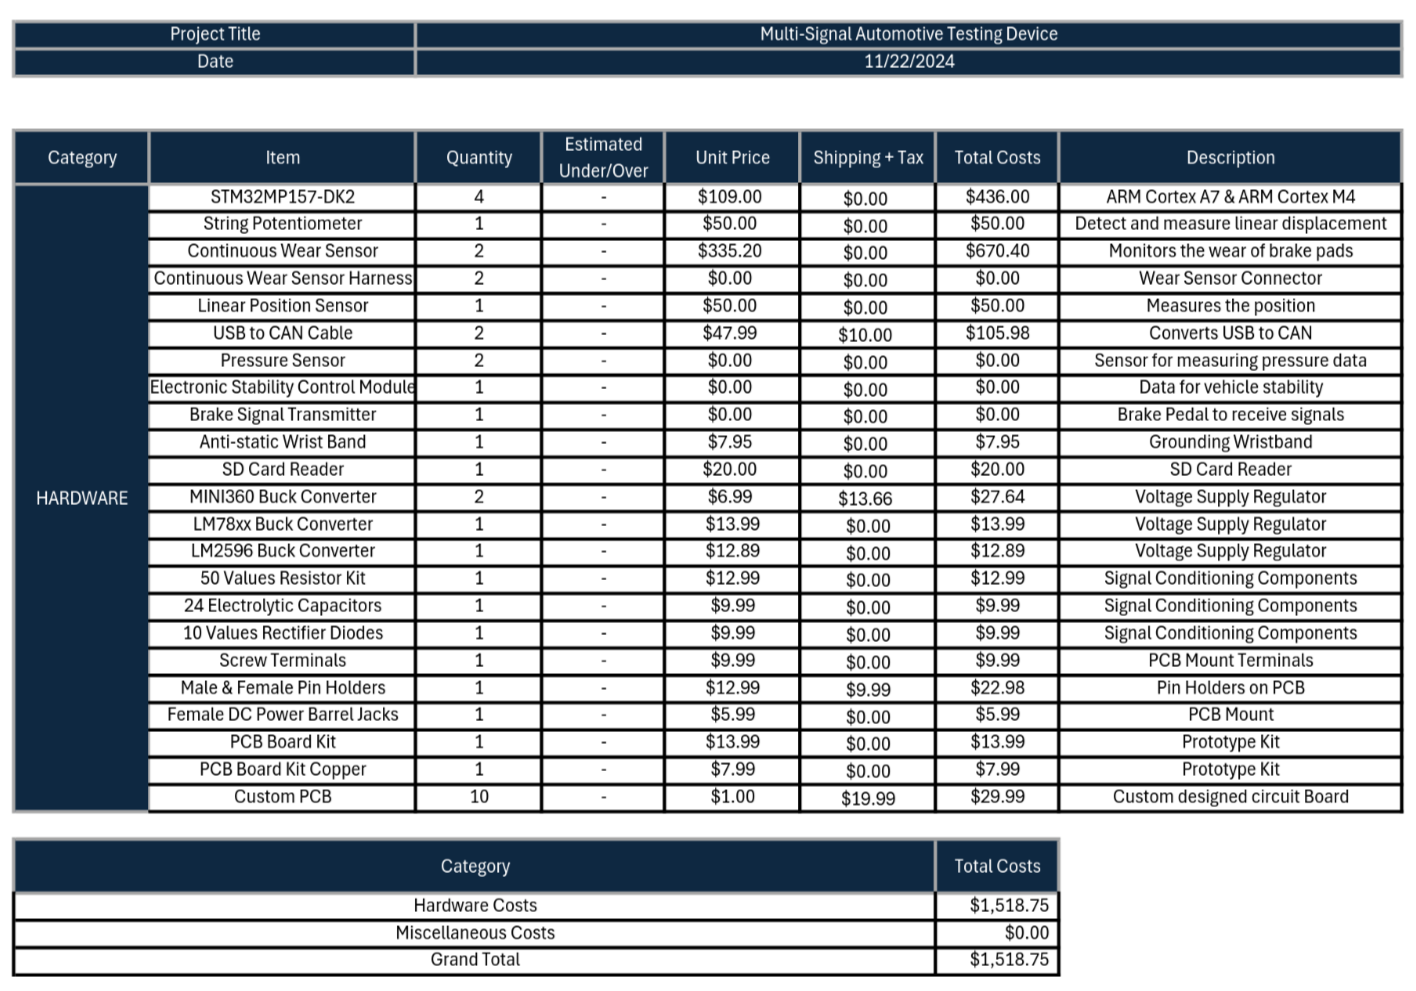
\includegraphics[height=0.675\textwidth]{assets/diagrams/budget.png}
\end{frame}

\AtBeginSubsection[]
{
  \begin{frame}
    \frametitle{Table of Contents}
    \tableofcontents[currentsubsection]
  \end{frame}
}

%==============================================================================
% DESIGN AND IMPLEMENTATION SECTION: Hardware Design
%==============================================================================
\begin{frame}
  \frametitle{Peripheral Schematic Design}
  \begin{block}{Overview}
    \begin{itemize}
      \item The schematic illustrates the design for connecting the devices under test (DUTs) to the STM32-DK2 microcontroller.
    \end{itemize}
  \end{block}
  \begin{block}{Key Design Elements}
    \begin{itemize}
      \item Signal Conditioning Circuits
      \item Resistors for voltage scaling, current limiting, and signal stabilization.
      \item Diodes to protect against voltage spikes and reverse polarity.
    \end{itemize}
  \end{block}
\end{frame}

\subsection{Hardware Design}
\begin{frame}
  \frametitle{Power Supply Schematic Design}
  \begin{minipage}{0.7\textwidth}
    \begin{figure}
      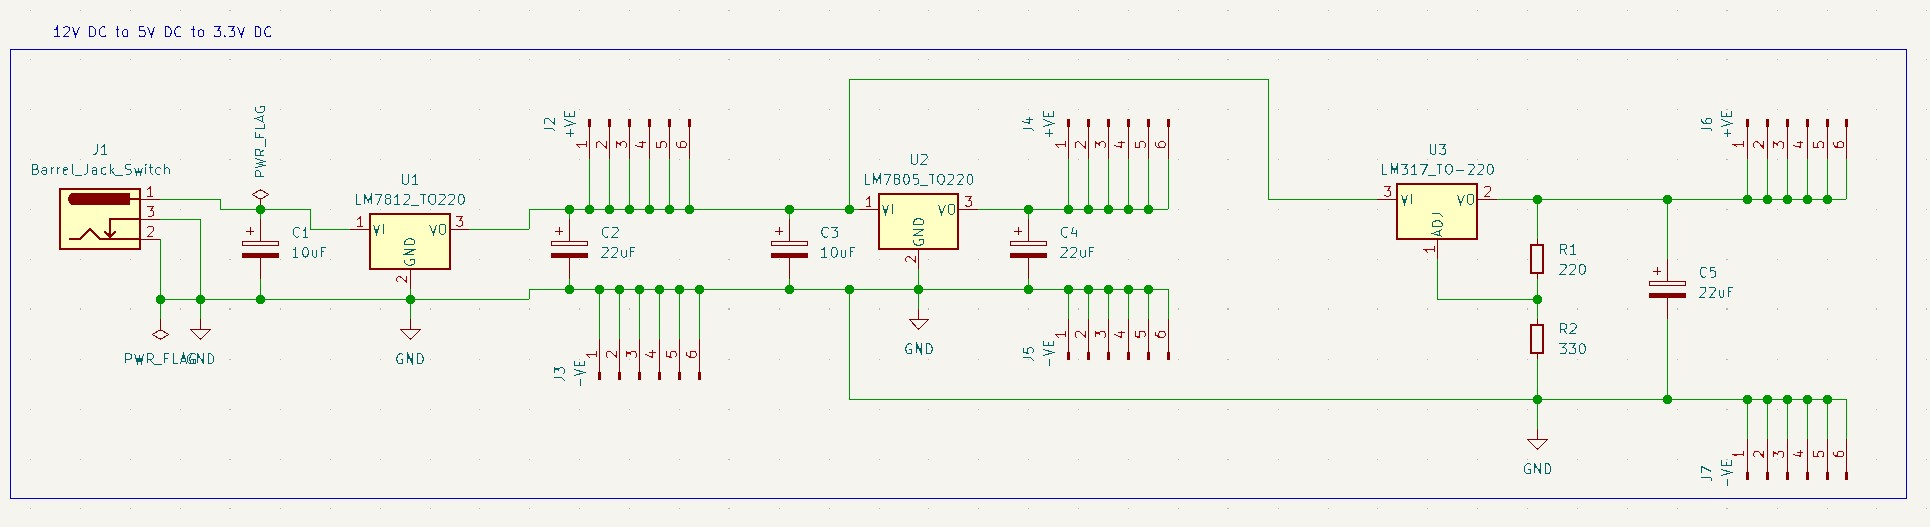
\includegraphics[width=\textwidth]{assets/electronic/pwrsupply.jpg}
      \caption{\it power management system that converts 12V DC input into multiple usable voltage levels.}
    \end{figure}
  \end{minipage}
  \hfill
  \begin{minipage}{0.275\textwidth}
    \begin{block}{Overview}
      \begin{itemize}
          \small
        \item 12V DC stable voltage using LM7812 (1A)
        \item 12V to 5V DC using LM7805 (1A)
        \item 12V to 3.3V using LM317 adjustable regulator
      \end{itemize}
    \end{block}
    \begin{block}{Key Components}
      \begin{itemize}
          \small
        \item LM7812, LM7805, LM317 voltage regulators for step-down conversion.
        \item Capacitors for noise filtration.
        \item Resistors to set voltages for LM317 as 3.146V DC (50uA).
      \end{itemize}
    \end{block}
  \end{minipage}
\end{frame}

\begin{frame}
  \frametitle{Schematic Design - Brake Signal Transmitter  }
  \begin{minipage}{0.6\textwidth}
    \begin{figure}
      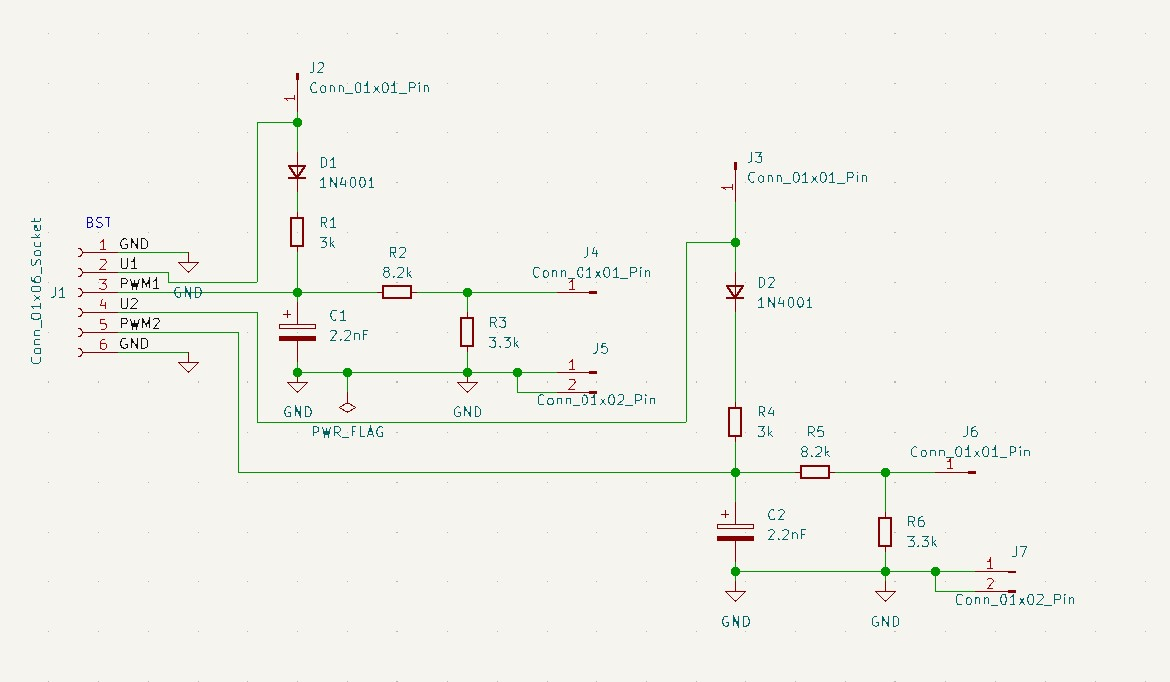
\includegraphics[width=\textwidth]{assets/electronic/bst_schem.jpg}
    \end{figure}
  \end{minipage}
  \hfill
  \begin{minipage}{0.375\textwidth}
    \begin{itemize}
      \begin{block}{(12V <50mA)}
        \item Reads PWM signals and wake-up signals
        \item Includes resistors and capacitors for signal filtering
      \end{block}
    \end{itemize}
  \end{minipage}
\end{frame}

\begin{frame}
  \frametitle{Continuous Wear Sensor (5V/<25mA)}
  \begin{minipage}{0.65\textwidth}
    \begin{figure}
      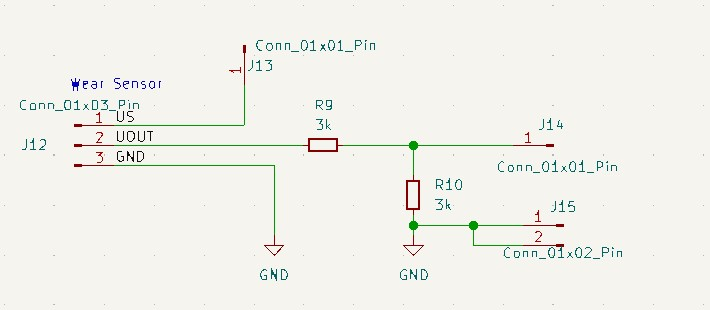
\includegraphics[width=\textwidth]{assets/electronic/wear_schem.jpg}
    \end{figure}
  \end{minipage}
  \hfill
  \begin{minipage}{0.3\textwidth}
    \begin{block}{Key Points}
      \begin{itemize}
        \item Captures analog voltage  to monitor brake wear.
        \item Uses voltage dividers for safe microcontroller input levels.
      \end{itemize}
    \end{block}
  \end{minipage}
\end{frame}

\begin{frame}
  \frametitle{Pressure Sensor (12V <15ma)}
  \begin{minipage}{0.65\textwidth}
    \begin{figure}
      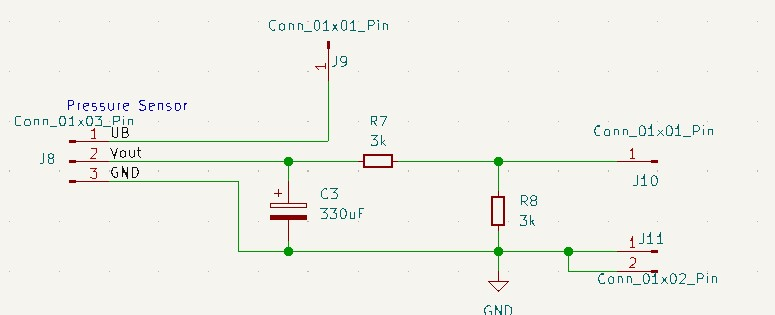
\includegraphics[width=\textwidth]{assets/electronic/pressure_schem.jpg}
    \end{figure}
  \end{minipage}
  \hfill
  \begin{minipage}{0.3\textwidth}
    \begin{block}{Key Points}
      \begin{itemize}
        \item Reads analog signals proportional to pressure.
        \item Includes voltage dividers for safe microcontroller input levels.
        \item Uses capacitors to stabilize the output.
      \end{itemize}
    \end{block}
  \end{minipage}
\end{frame}

\begin{frame}
  \frametitle{String Potentiometer  (12V/<20mA)}
  \begin{minipage}{0.65\textwidth}
    \begin{figure}
      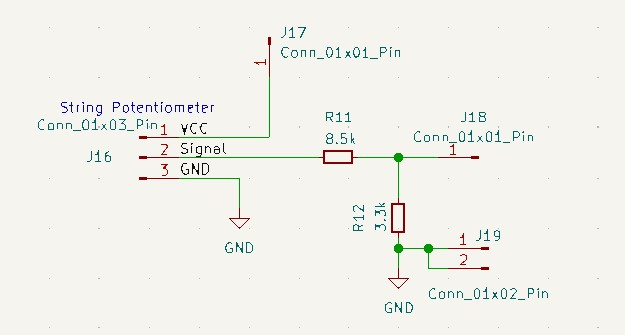
\includegraphics[width=\textwidth]{assets/electronic/string_pcb.jpg}
    \end{figure}
  \end{minipage}
  \hfill
  \begin{minipage}{0.3\textwidth}
    \begin{block}{Key Points}
      \begin{itemize}
        \item Converts displacement into proportional analog voltage.
        \item Includes resistors as voltage dividers for scaling and conditioning.
      \end{itemize}
    \end{block}
  \end{minipage}
\end{frame}

\begin{frame}
  \frametitle{Printed Circuit Board Design}
  \begin{minipage}{0.3\textwidth}
    \begin{figure}
      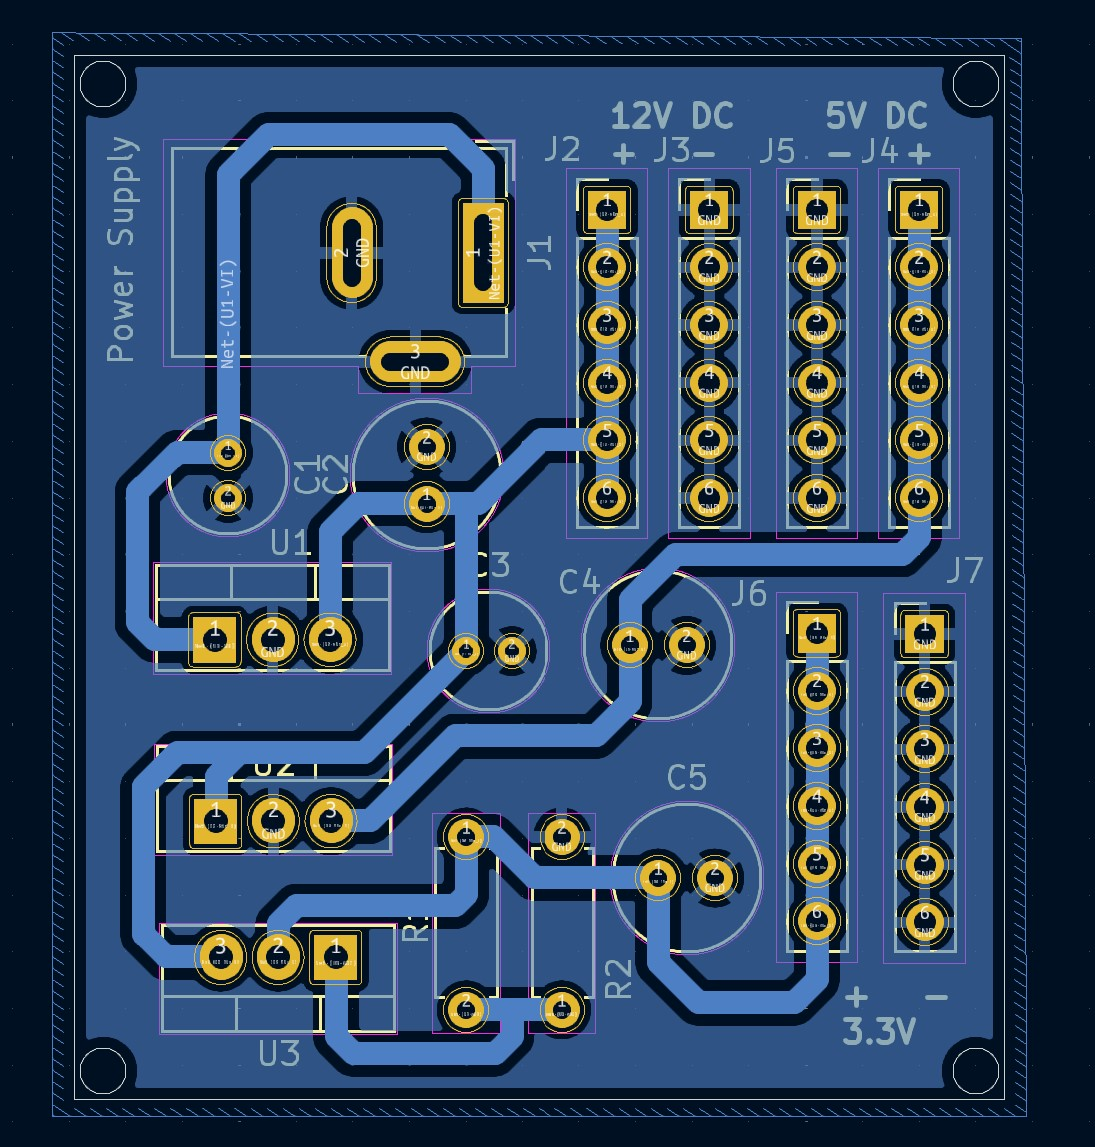
\includegraphics[width=\textwidth]{assets/electronic/pwrsupply_pcb.jpg}
    \end{figure}
  \end{minipage}
  \hfill
  \begin{minipage}{0.675\textwidth}
    \begin{block}{Overview}
      \begin{itemize}
          \small
        \item The power supply PCB converts the 12V DC input from the DC jack into regulated output voltages for the system.
          \begin{itemize}
              \tiny
            \item  12V DC
            \item 5V DC
            \item 3.3V DC
          \end{itemize}
        \item It is designed based on the schematic with components such as voltage regulators (LM7812, LM7805, LM317), capacitors, and resistors.
      \end{itemize}
    \end{block}
    \begin{block}{Key Components}
      \begin{itemize}
          \footnotesize
        \item DC Jack (J1): Connects the input 12V DC power supply to the board.
        \item Output Pins:
          \begin{itemize}
              \tiny
            \item J2/J3: Provides 12V DC output.
            \item J4/J5: Provides 5V DC output.
            \item J6/J7: Provides 3.3V DC output.
          \end{itemize}
        \item Voltage Regulators
          \begin{itemize}
              \tiny
            \item Step-down conversion for different voltage levels.
            \item Smooth and stable output.
          \end{itemize}
        \item Capacitors (C1-C5)
          \begin{itemize}
              \tiny
            \item Ensure smooth voltage output by filtering noise and ripples.
          \end{itemize}
        \item Ground connections: All components are referenced to a common ground for stable operation.
      \end{itemize}
    \end{block}
  \end{minipage}
\end{frame}

\begin{frame}
  \frametitle{Peripherals Printed Circuit Board}
  \begin{minipage}{0.5\textwidth}
    \begin{block}{Key Features}
      \begin{itemize}
          \small
        \item Input/Power Pins:
          \begin{itemize}
              \footnotesize
            \item Each DUT has a dedicated connector for input signals and a power signal.
            \item J1: Inputs for BST (PWM1 and PWM2) | J2/J3: 12V Power Signals for BST (PWM1 and PWM2)
            \item J8: Pressure sensor input | J9: 12V DC Power Signal
            \item J12: Wear sensor input | J13: 5V DC Power Signal
            \item J16: String Potentiometer input | J17: 12V DC Power signal
          \end{itemize}
        \item Output Pins:
          \begin{itemize}
              \footnotesize
            \item Processed signals are sent to the microcontroller through the output pins.
            \item J4/J5/J6/J7: BST processed signals
            \item J10/J11: Pressure sensor output
            \item J14/J15: Wear sensor output
            \item J18/J19: String potentiometer output.
          \end{itemize}
        \item Signal Conditioning:
          \begin{itemize}
              \footnotesize
            \item Resistors: Scale signals for safe microcontroller input.
            \item Capacitors: Filter noise and stabilize signals.
            \item Capacitors: Filter noise and stabilize signals.
          \end{itemize}
      \end{itemize}
    \end{block}
  \end{minipage}
  \hfill
  \begin{minipage}{0.45\textwidth}
    \begin{figure}
      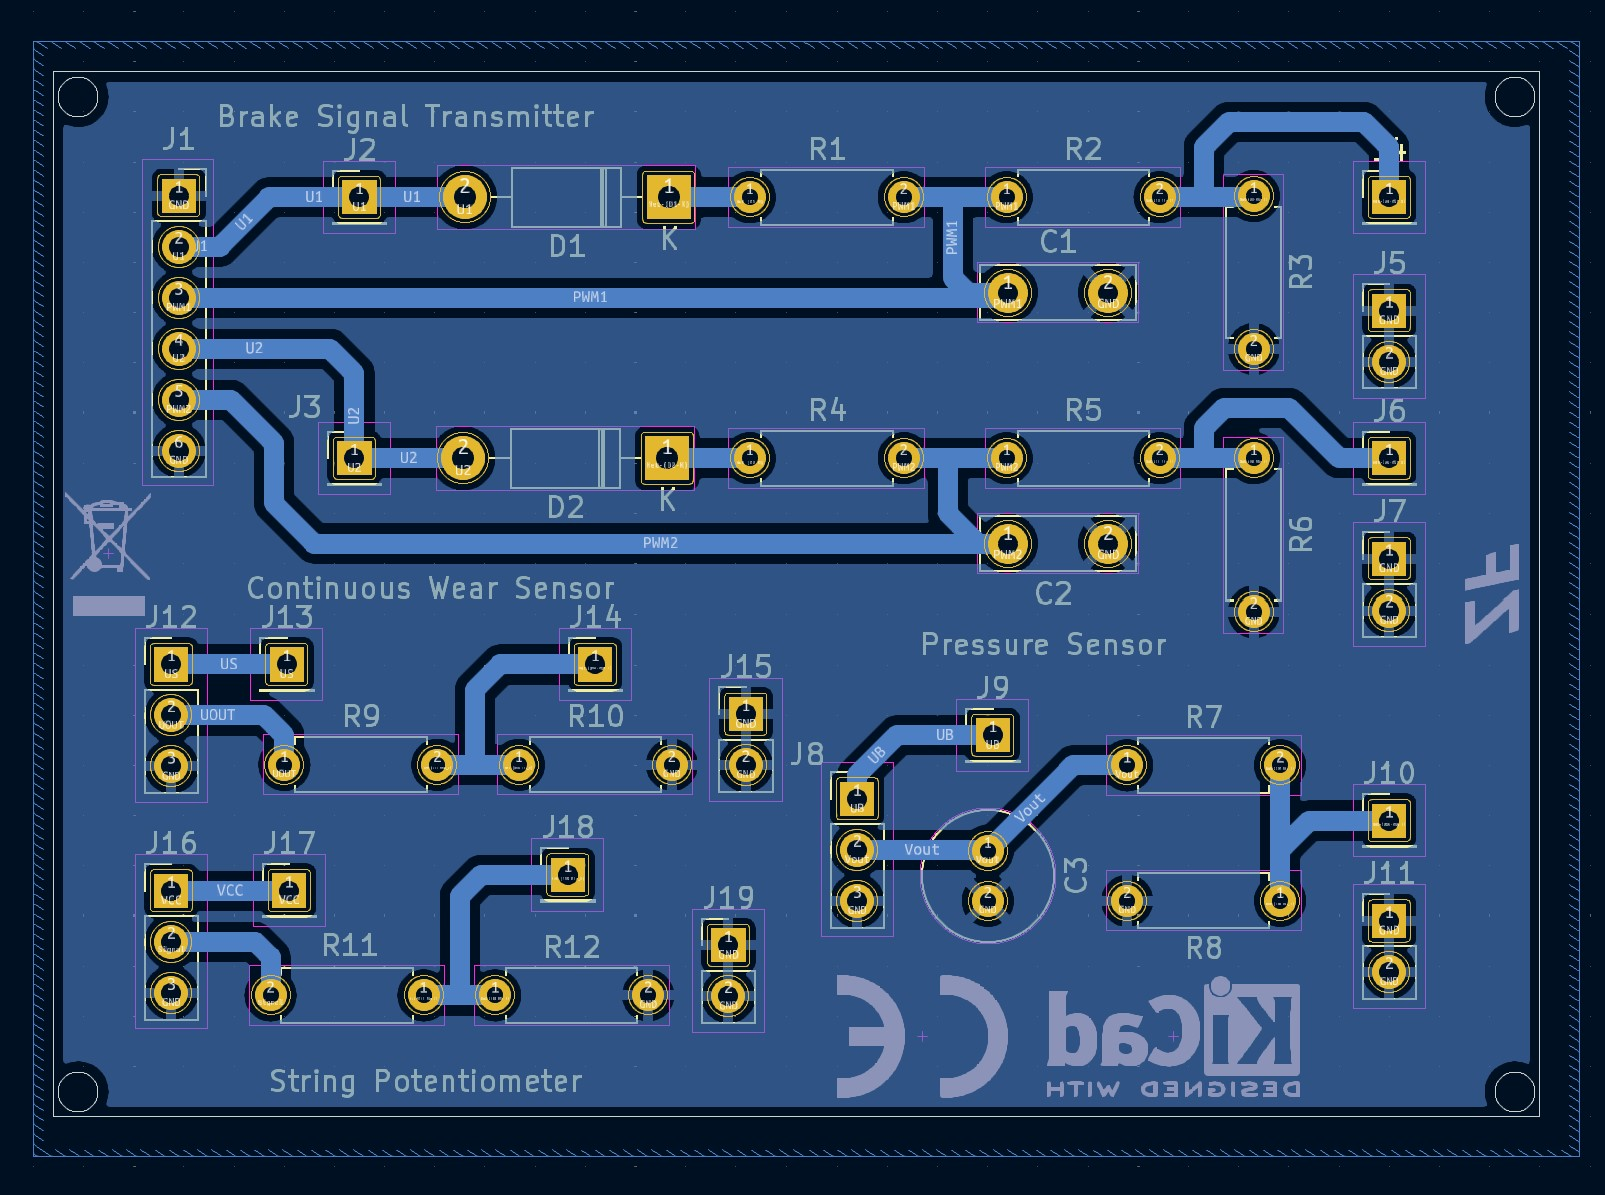
\includegraphics[width=\textwidth]{assets/electronic/peri_pcb.jpg}
    \end{figure}
  \end{minipage}
\end{frame}

\begin{frame}
  \frametitle{Fabricated PCB}
  \begin{minipage}{0.5\textwidth}
    \begin{figure}
      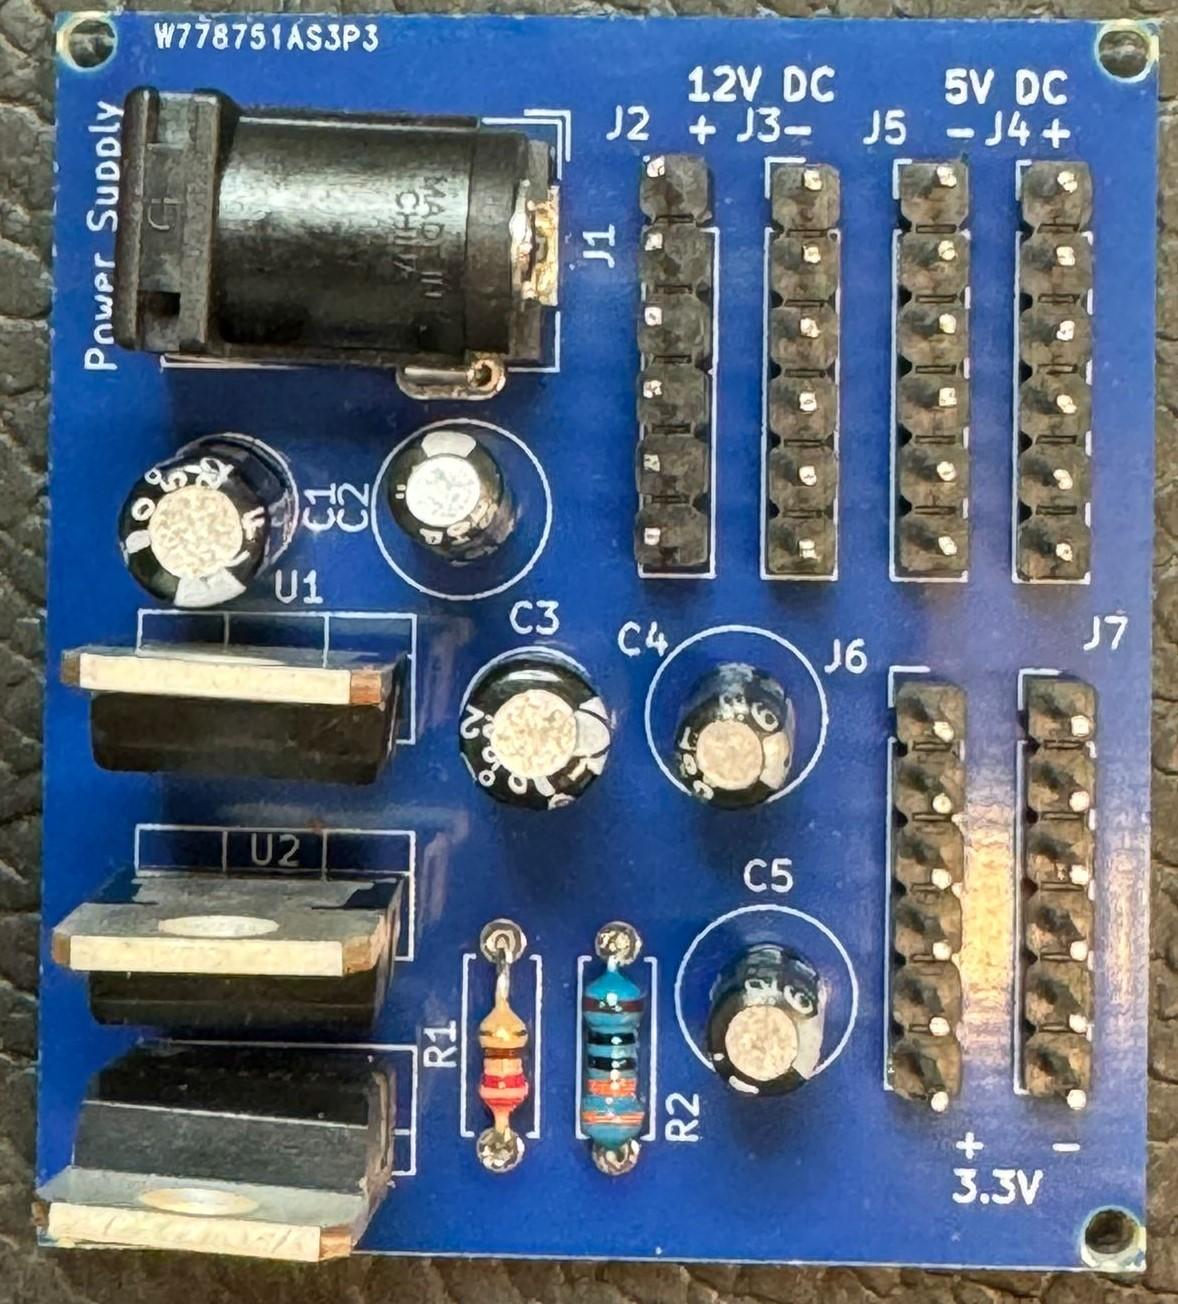
\includegraphics[width=\textwidth]{assets/electronic/pcb1.jpeg}
    \end{figure}
  \end{minipage}
  \hfill
  \begin{minipage}{.475\textwidth}
  \begin{figure}
    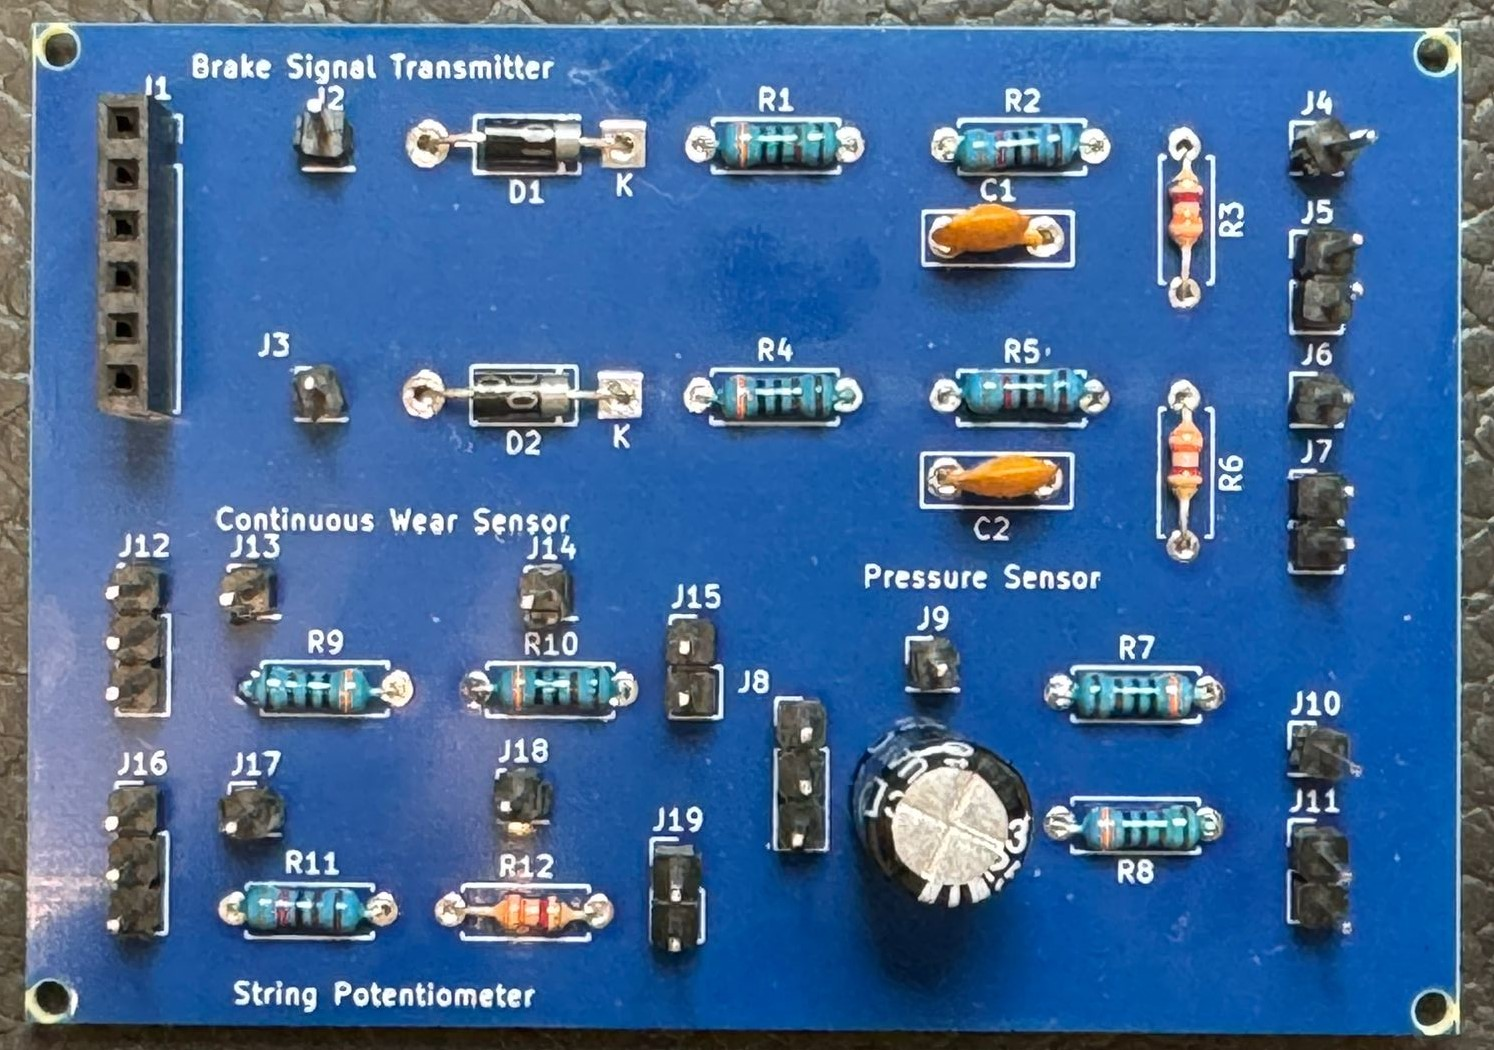
\includegraphics[width=\textwidth]{assets/electronic/pcb2.jpeg}
  \end{figure}
  \end{minipage}
\end{frame}

\begin{frame}
  \frametitle{Enclosure Design}
  \begin{minipage}{0.475\textwidth}
    \begin{figure}
      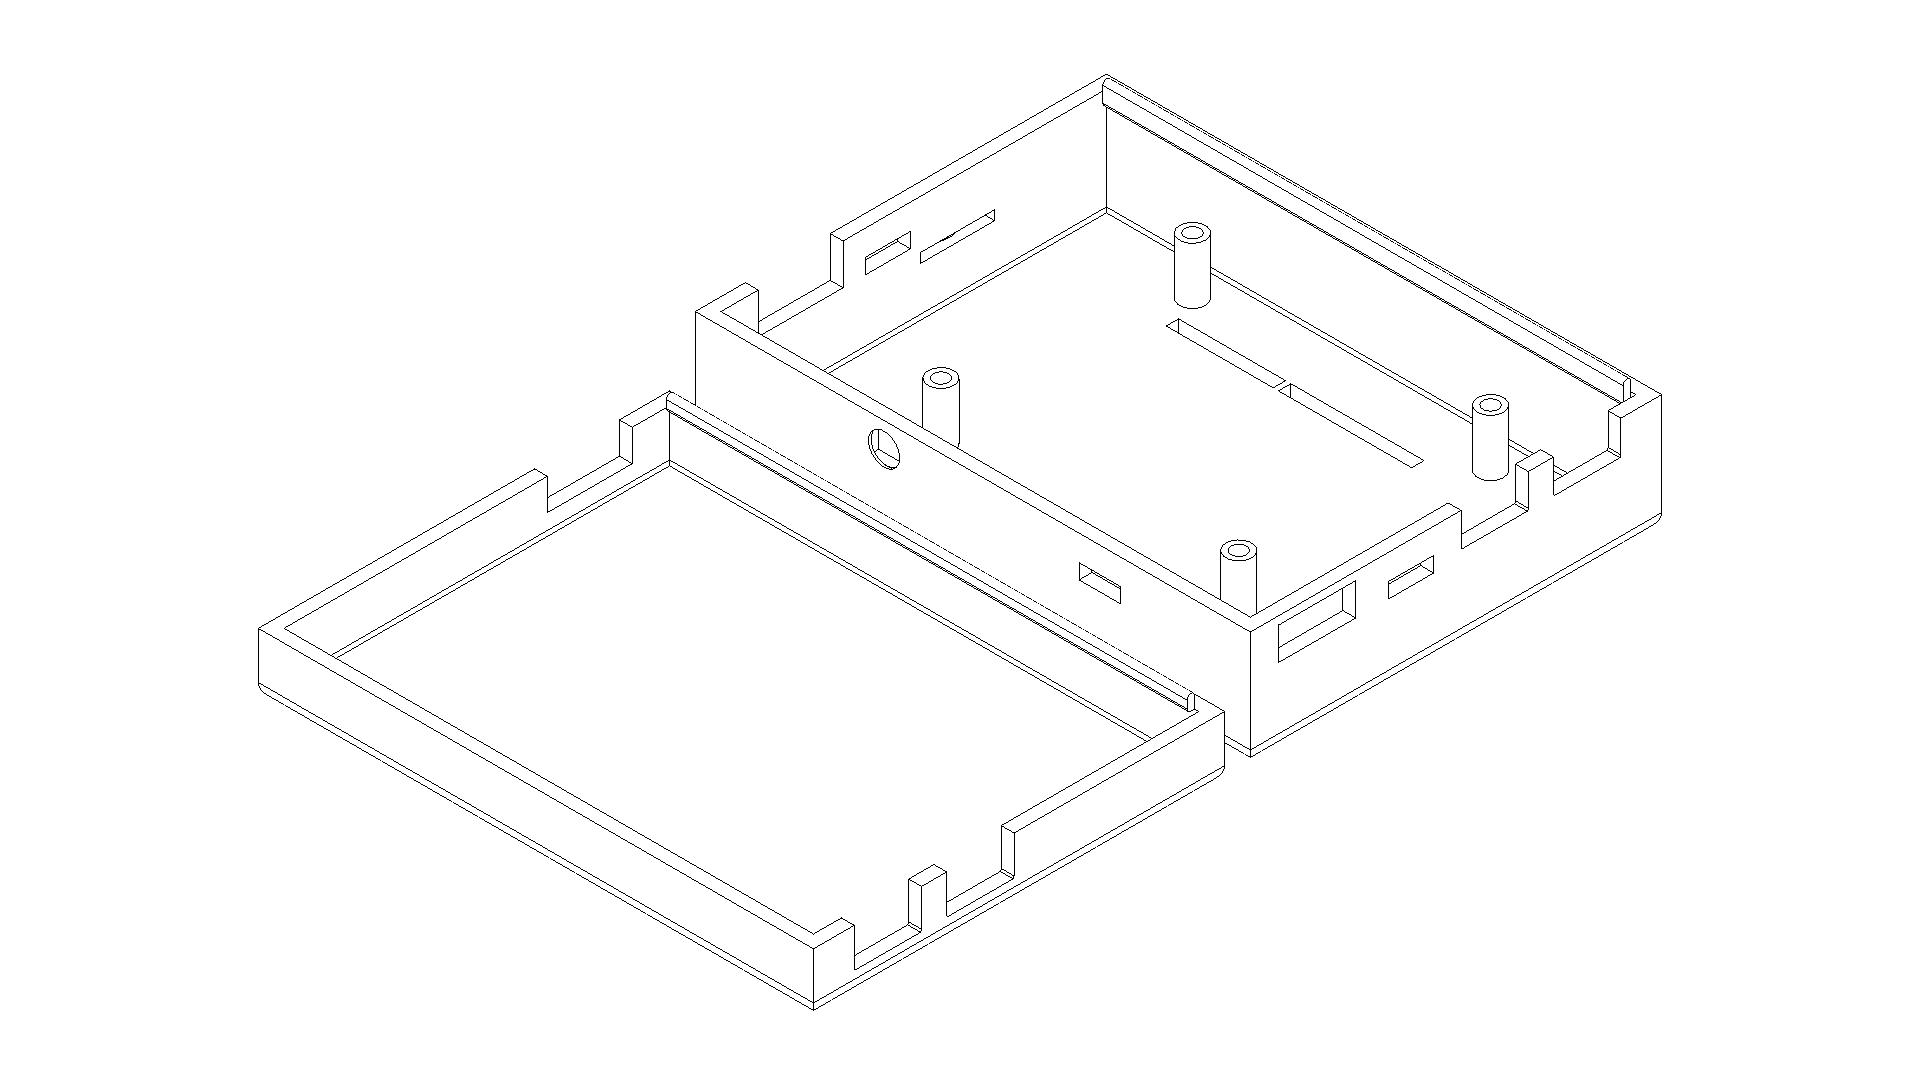
\includegraphics[width=\textwidth]{assets/electronic/stm32_enclosure_final_test_pic1.jpg}
      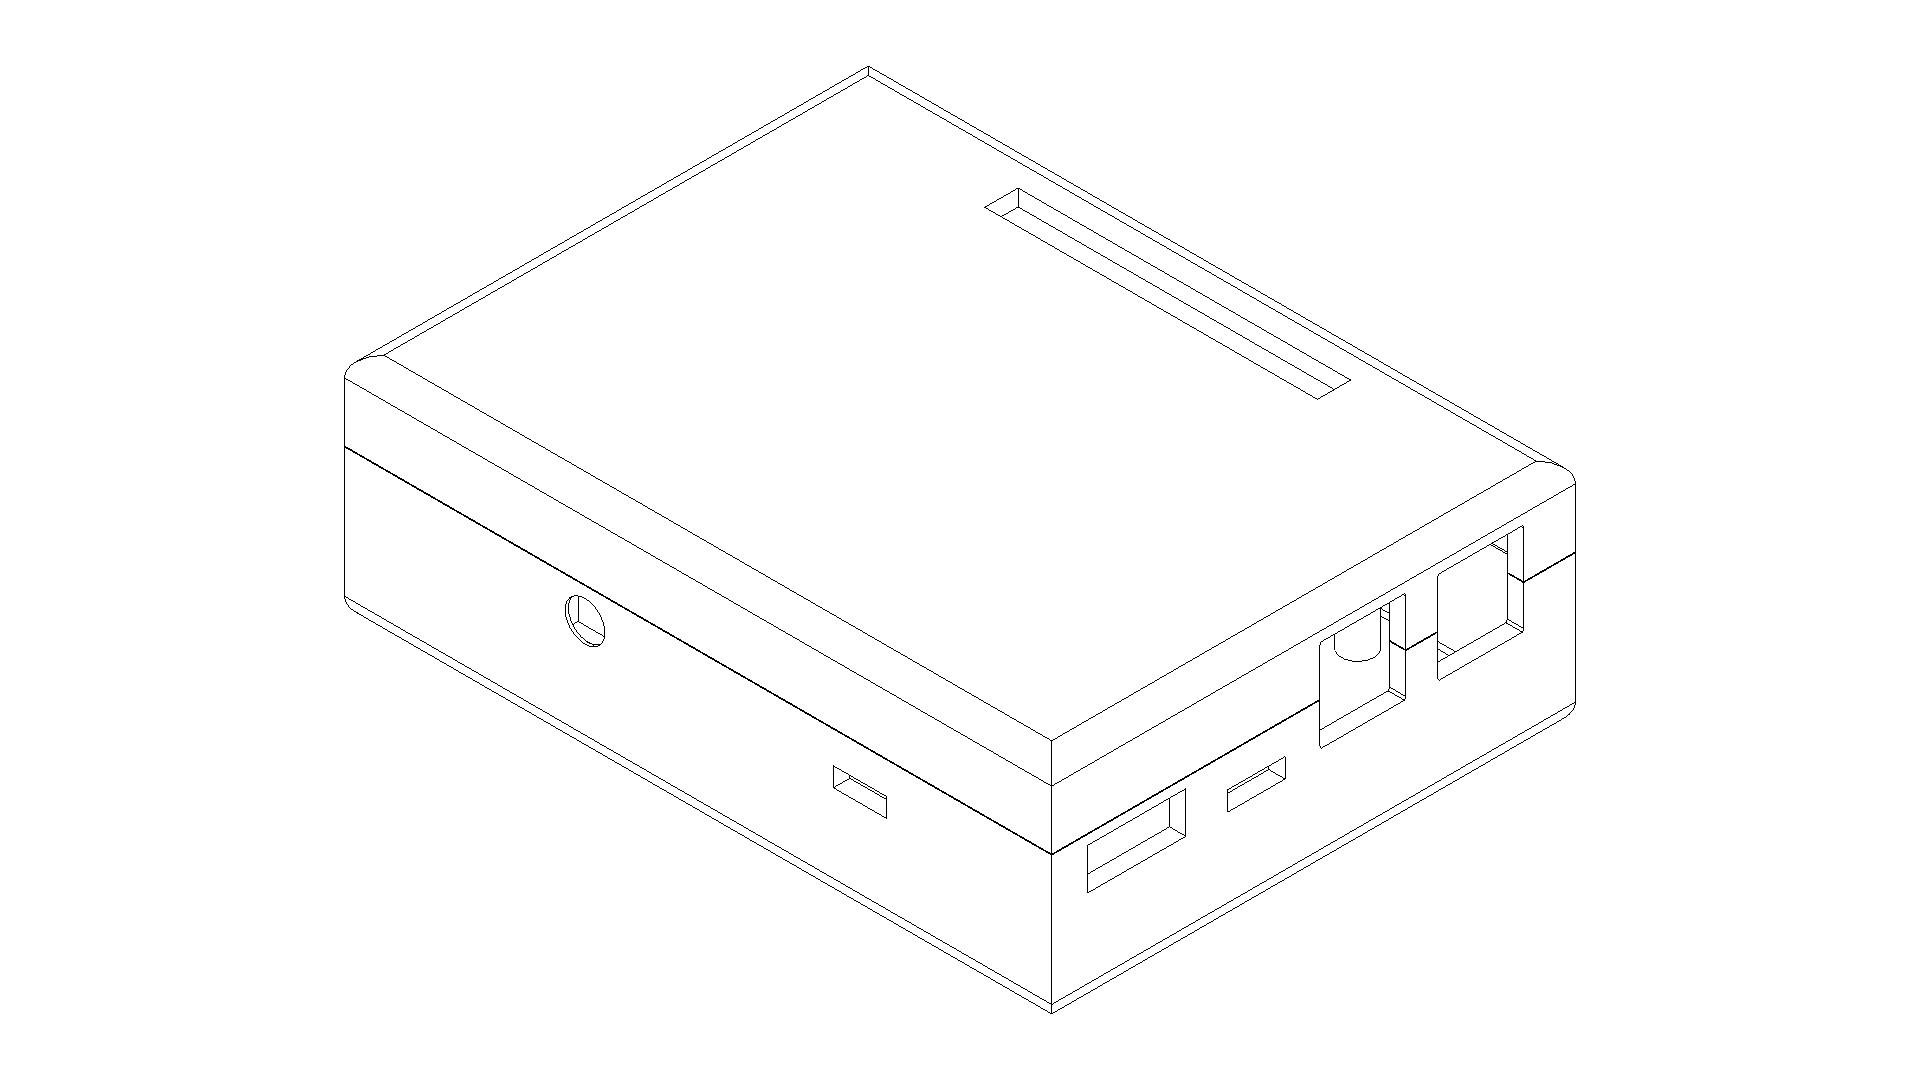
\includegraphics[width=\textwidth]{assets/electronic/stm32_enclosure_final_testpic2.jpg}
      \caption{\it Enclosure for STM32MP157F-DK2}
    \end{figure}
  \end{minipage}
  \hfill
  \begin{minipage}{0.45\textwidth}
    \begin{figure}
      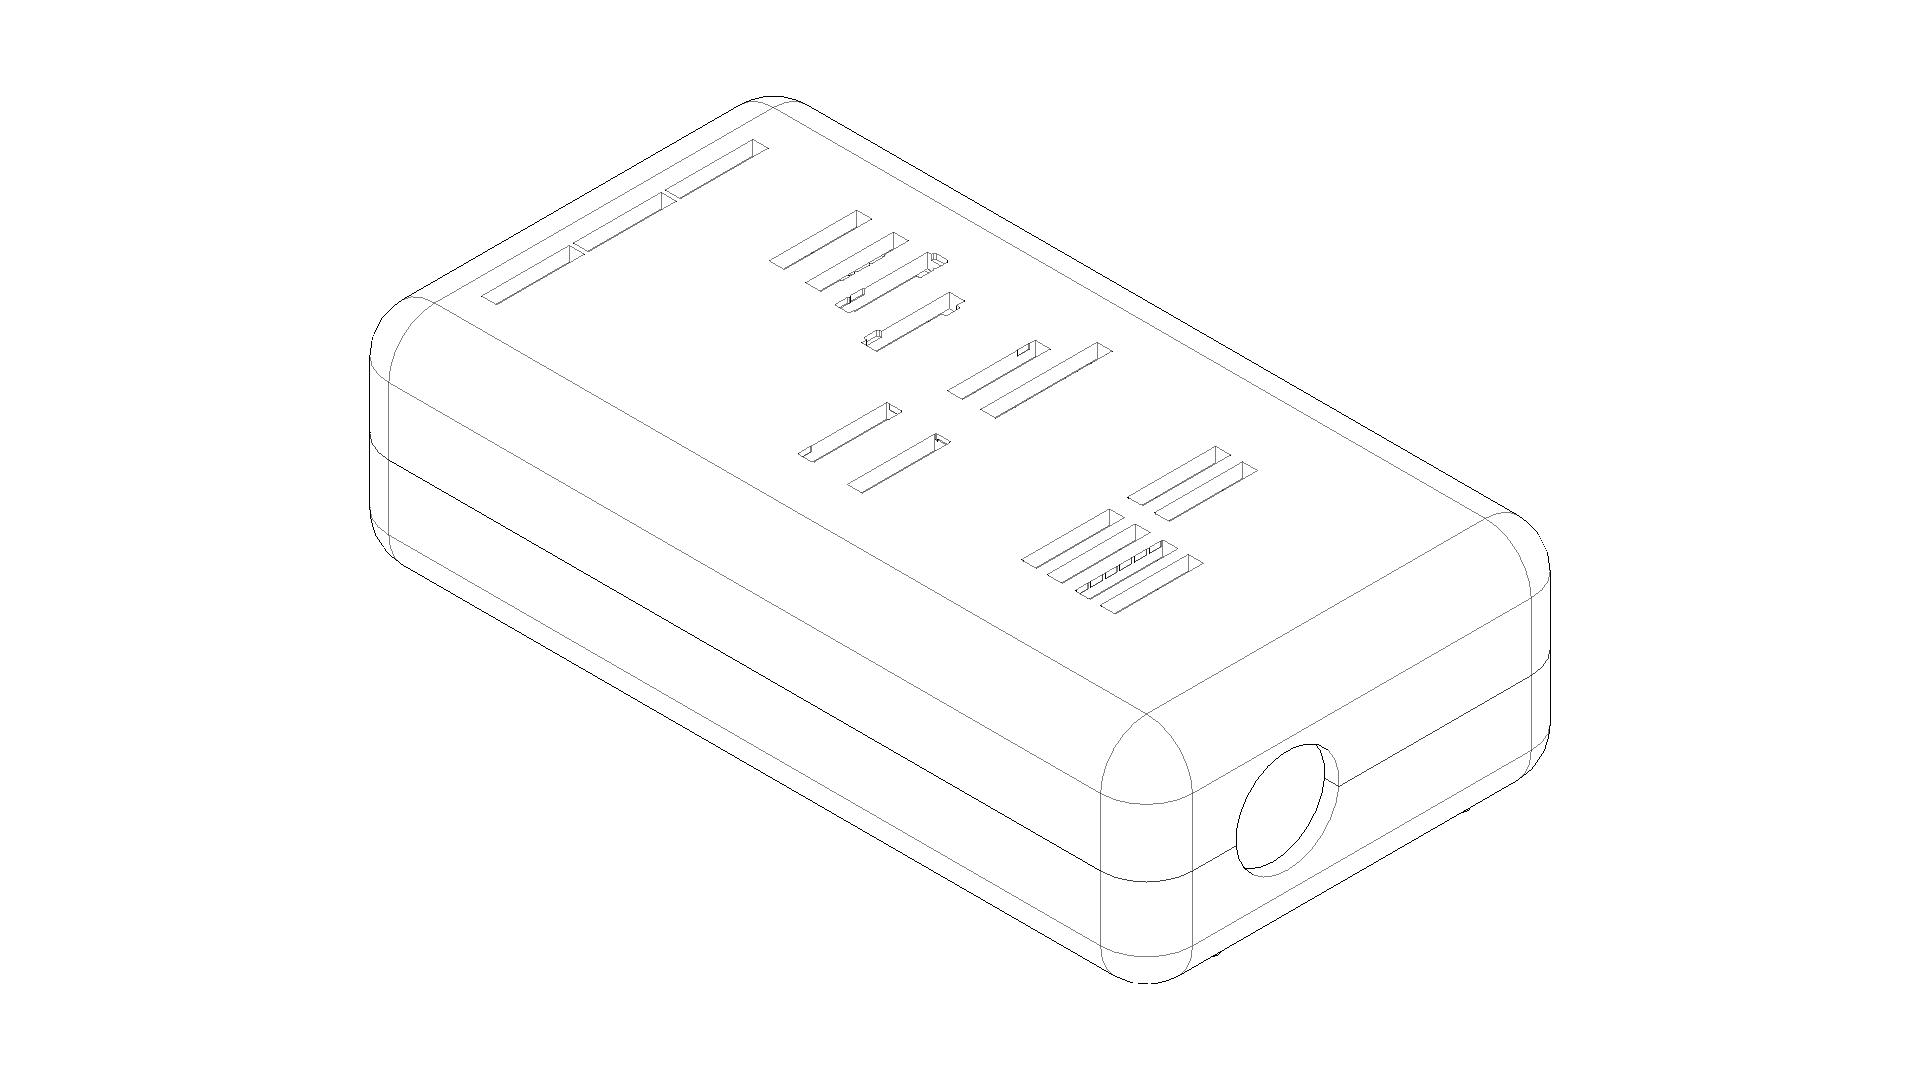
\includegraphics[width=\textwidth]{assets/electronic/psperi_enclosure_final_testpic1.jpg}
      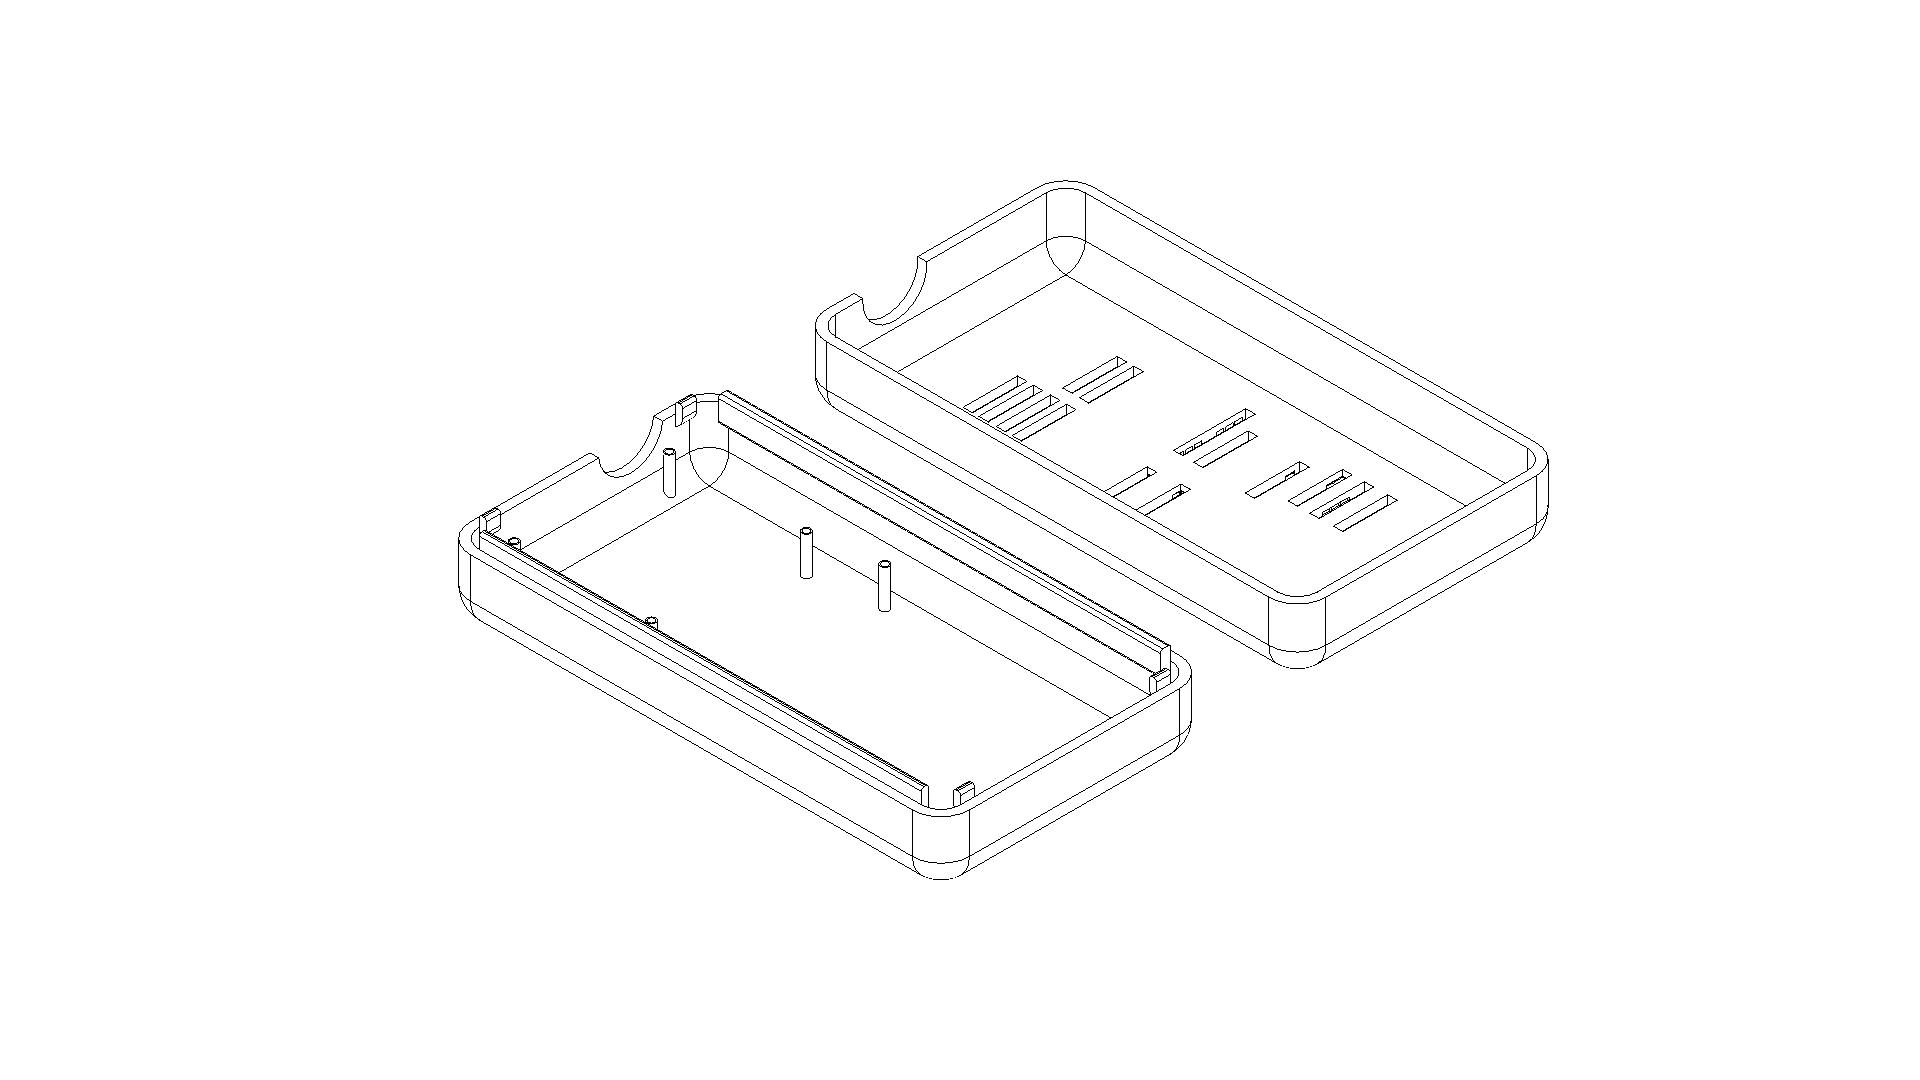
\includegraphics[width=\textwidth]{assets/electronic/psperi_enclosure_final_testpic2.jpg}
      \caption{\it Enclosure for PCBs}
    \end{figure}
  \end{minipage}
\end{frame}

%==============================================================================
% DESIGN AND IMPLEMENTATION SECTION: Cortex-M4 Firmware
%==============================================================================
\subsection{Device Interfacing and Testing}
\begin{frame}
  \frametitle{Firmware to Test Brake Signal Transmitter (BST)}
  \begin{block}{Purpose}
    \small{
      \begin{itemize}
        \item Developed firmware on the onboard Cortex-M4 microcontroller to validate BST
        \item Ensures brake actuation is accurate to distance moved by brake pedal
        \item \LightBold{Key Specifications:} Output range 1 mm to 9 mm, Sensitivity 5.96\% DC/mm, Output signals PWM1 and PWM2 (S1 and S2)
       % ^suggested change
      \end{itemize}
    }
  \end{block}
  \hspace{-0.5cm}
  \begin{minipage}{0.485\textwidth}
    \begin{block}{Method}
      \small{
        \begin{itemize}
          \item \LightBold{Input Capture:} Timers captures read two PWM signals from the BST
          \item \LightBold{ADC Reading:}Optional string potentiometer for direct analog voltage measurements via ADC 
            %^ADC already defined in project specification, "converter" after ADC is redundant
          \item \LightBold{Processing:} Calculates duty cycles, frequencies, and estimated stroke via timer interrupts
            %^changed "readings" to "interrupts"
          \item \LightBold{Validation:} Compare measurements against expected values according to product specifications to verify BST accuracy
          \item \LightBold{Results:} Sends test results to the main processor for logging and user display
        \end{itemize}
      }
    \end{block}
  \end{minipage}
  \hfill
  \begin{minipage}{0.50\textwidth}
    \begin{figure}
      \centering
      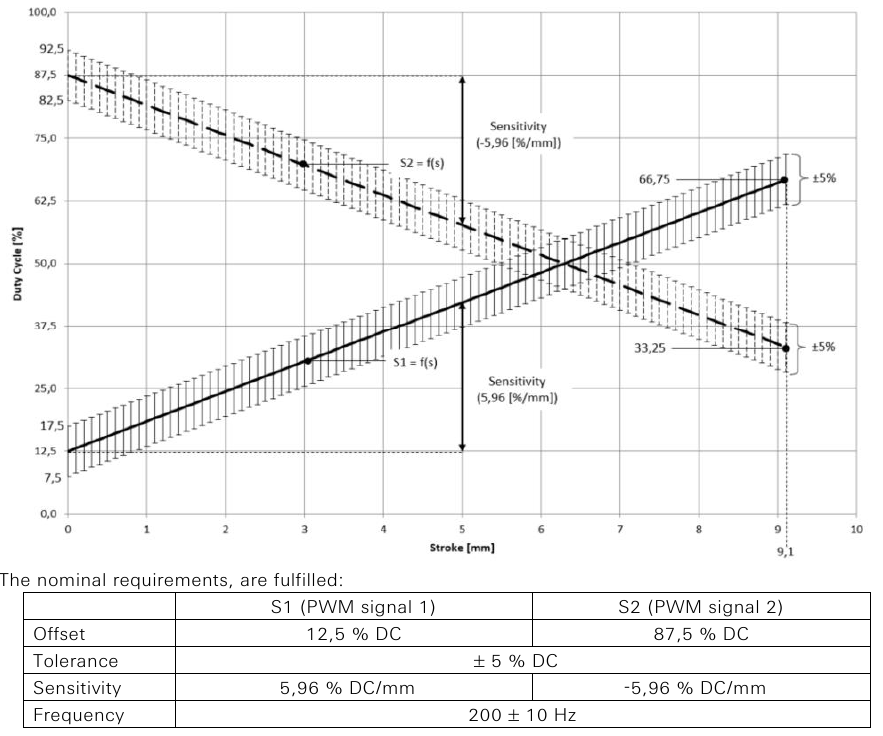
\includegraphics[width=\textwidth]{assets/specs/bst_product_specs.png}
      \caption{\it Product Specifications for BST}
    \end{figure}
  \end{minipage}
\end{frame}

% CWS Test implementation
\begin{frame}
    \frametitle{Firmware to Test Continuous Wear Sensor (CWS)}
    \begin{block}{Purpose}
        \small{
            \begin{itemize}
                \item Developed firmware on the onboard Cortex-M4 microcontroller to validate the Continuous Wear Sensor (CWS)
                \item Ensures accurate measurement of brake pad wear levels to enhance vehicle safety
                \item \LightBold{Key Specifications:} Output range 0.7V (18 mm or new pad) to 4.0 V (53 mm or worn pad), Sensitivity 0.08 V/mm, Voltage divider ratio 2:1
            \end{itemize}
        }
    \end{block}
    \hspace{-0.5cm}
    \begin{minipage}{0.485\textwidth}
        \begin{block}{Method}
            \small{
                \begin{enumerate}
                    \tiny
                    \item \LightBold{ADC Configuration:} Read direct analog voltage via ADC using DMA for efficiency and a timer trigger for consistency
                    \item \LightBold{Wear Calculation:} Mapped the measured voltage to brake pad wear using a linear relationship and handled special conditions (e.g., new pad, worn-out pad) with specific tolerances
                    \item \LightBold{Validation:} Compared wear values against expected values based on product specifications
                    \item \LightBold{Results:} Error thresholds to determine pass/fail and send detailed test outcomes to the main processor for logging and user display
                \end{enumerate}
            }
        \end{block}
    \end{minipage}
    \hfill
    \begin{minipage}{0.50\textwidth}
        \begin{figure}
            \centering
            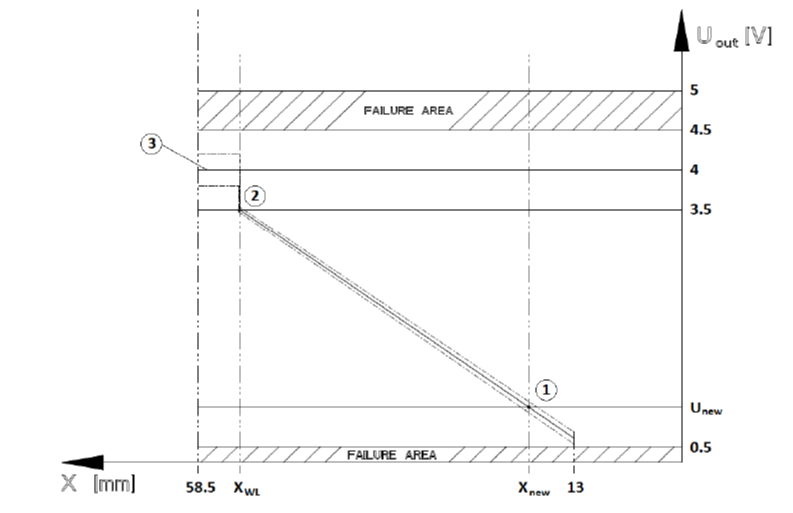
\includegraphics[width=\textwidth]{assets/specs/cws_product_specs.png}
            \caption{\it Product Specifications for CWS}
        \end{figure}
        \vspace{0.2cm}
    \end{minipage}
\end{frame}

% PS Test implementation
\begin{frame}
    \frametitle{Firmware to Test Pressure Sensor}
    \begin{block}{Purpose}
        \small{
            \begin{itemize}
                \item Developed firmware to validate Pressure Sensor readings on the Cortex-M4 microcontrooler
                \item Ensures accurate measurement of pressure when given for reliable vehicle control system purposes
                \item \LightBold{Key Specifications:} Output range 0.5V (0 bar) to 4.5 V (10 bar), Sensitivity 0.4 V/Bar, Voltage divider ratio 2:1
            \end{itemize}
        }
    \end{block}
    \hspace{-0.5cm}
    \begin{minipage}{0.485\textwidth}
        \begin{block}{Method}
            \small{
                \begin{enumerate}
                    \tiny
                    \item \LightBold{ADC Configuration:} Configured the ADC to read analog voltage from the Pressure Sensor using DMA for efficient data transfer and utilized a timer to trigger ADC conversions periodically
                    \item \LightBold{Pressure Calculation:} Mapped the measured voltage to pressure using a linear relationship given in the product specifications with the addition of converted pressure from bar to psi
                    \item \LightBold{Validation:} Compared calculated pressure against expected values based on product specifications with voltage tolerances to determine pass/fail status
                    \item \LightBold{Results:} Sent detailed test outcomes to the main processor for logging and user display
                \end{enumerate}
            }
        \end{block}
    \end{minipage}
    \hfill
    \begin{minipage}{0.50\textwidth}
        \begin{figure}
            \centering
            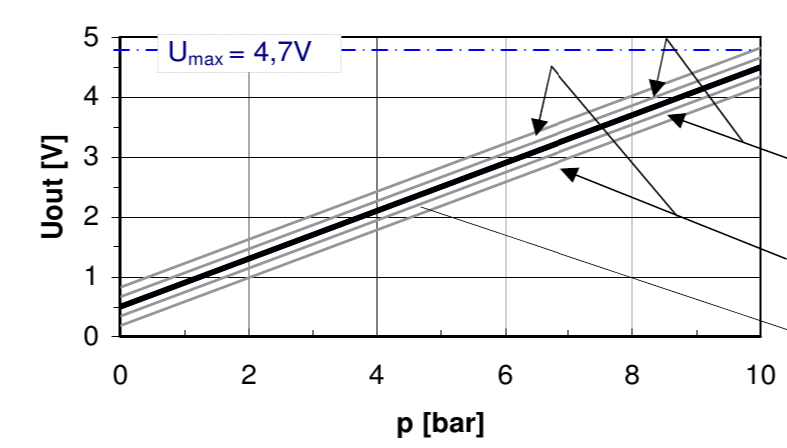
\includegraphics[width=\textwidth]{assets/specs/adc_product_specs.png}
            \caption{\it Product Specifications for CWS}
        \end{figure}
        \vspace{0.2cm}
    \end{minipage}
\end{frame}
%==============================================================================
% DESIGN AND IMPLEMENTATION SECTION: Embedded Linux
%==============================================================================
\subsection{Embedded Linux With Yocto Project}

% Consolidation slide to summarize the next two slides

\begin{frame}
  \frametitle{}
\end{frame}

\begin{frame}
  \frametitle{Embedded Linux}
  \begin{figure}
    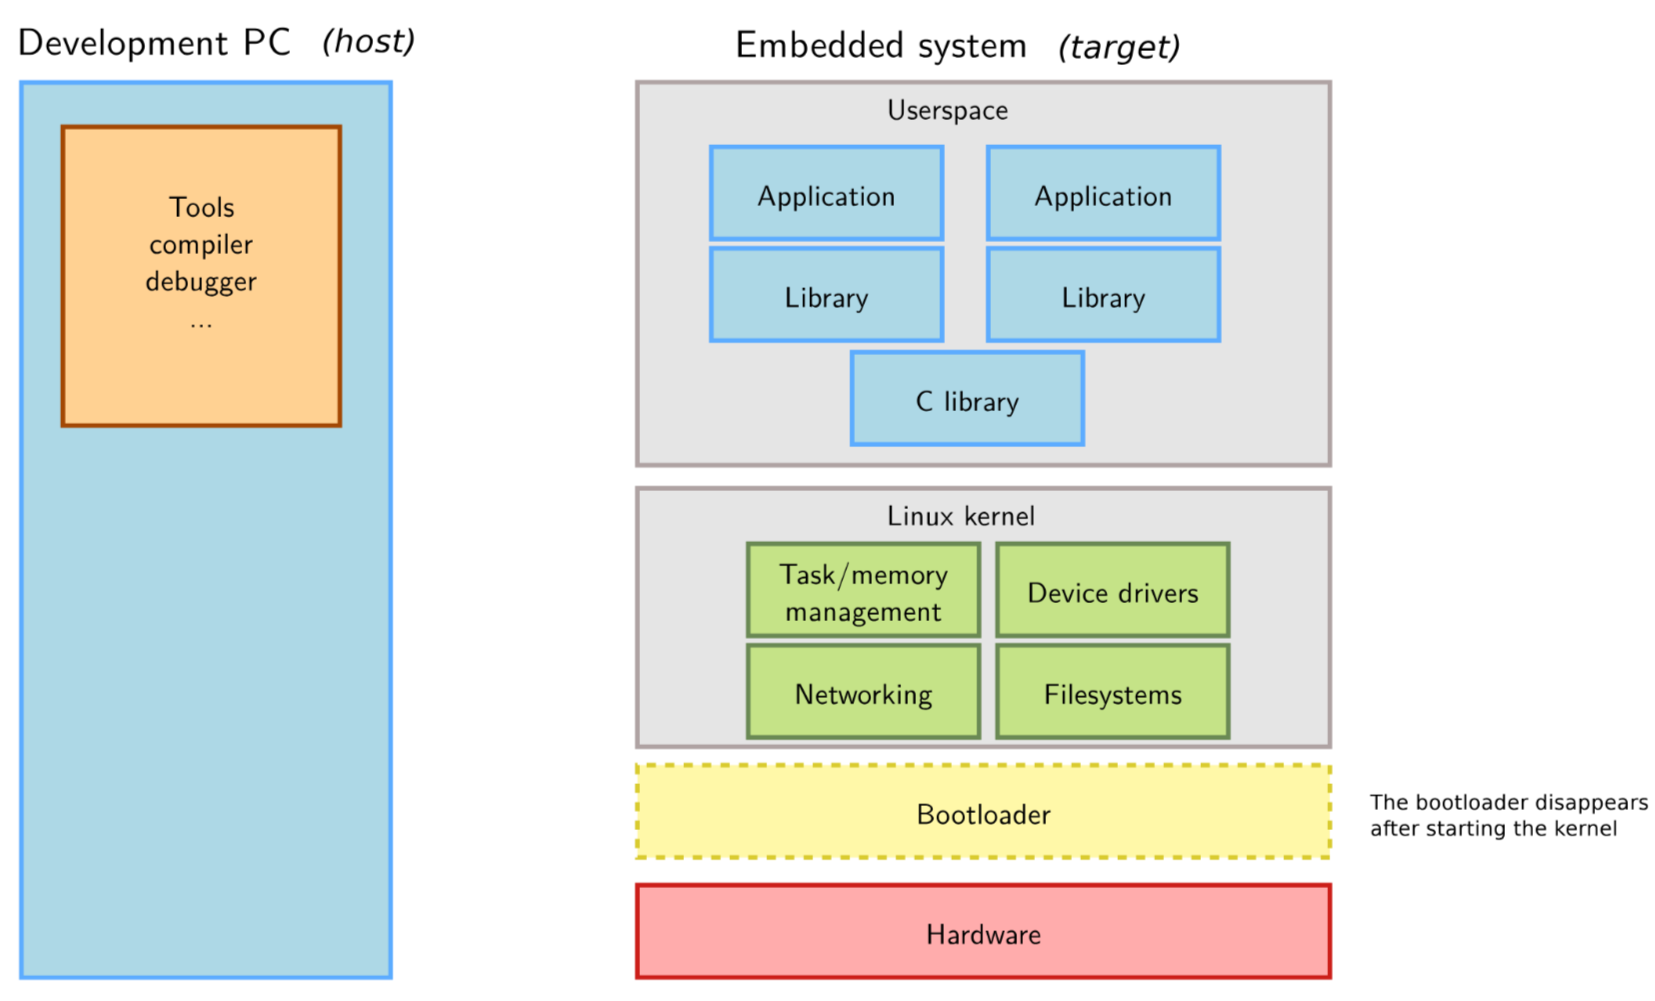
\includegraphics[width=175px]{assets/diagrams/embedded_linux.png}
    \centering
    \caption{\tiny Source:\underline{\href{https://bootlin.com/}{https://bootlin.com/}}\hspace{\textwidth}
    \textit{Embedded Linux system architecture}}
  \end{figure}
  \vspace{-16px}
  \begin{block}{Why use embedded Linux?}
    \small{
      \begin{itemize}
        \item Industry standard for any embedded operating system
        \item Access to open-source software (OSS) and tools
        \item Networking and connectivity made easy 
        \item Easily save/access data with filesystem
      \end{itemize}
    }
  \end{block}
\end{frame}

\begin{frame}
  \frametitle{Using The Yocto Project to Build a Custom Distribution}
    \begin{block}{What is the Yocto Project and why?}
      {
        \begin{itemize}
          \item Most popular set of tools for embedded Linux Development
          \item Collection of OSS tools to make a custom Linux distribution
          \item Independent of target architecture
          \item \DarkBoldP{bitbake} build tool handles \LightBold{metadata}
          \item \LightBold{MetaData} can be in the form of 
            \begin{itemize}
              \item software build/patch instructions
              \item configuration files for software
            \end{itemize}
          \item \LightBold{MetaData} organized in its \LightBold{Layer Model}
        \end{itemize}
      }
    \end{block}
  \hfill
    \vspace{-12px}
    \center
    \begin{figure}
      \center
      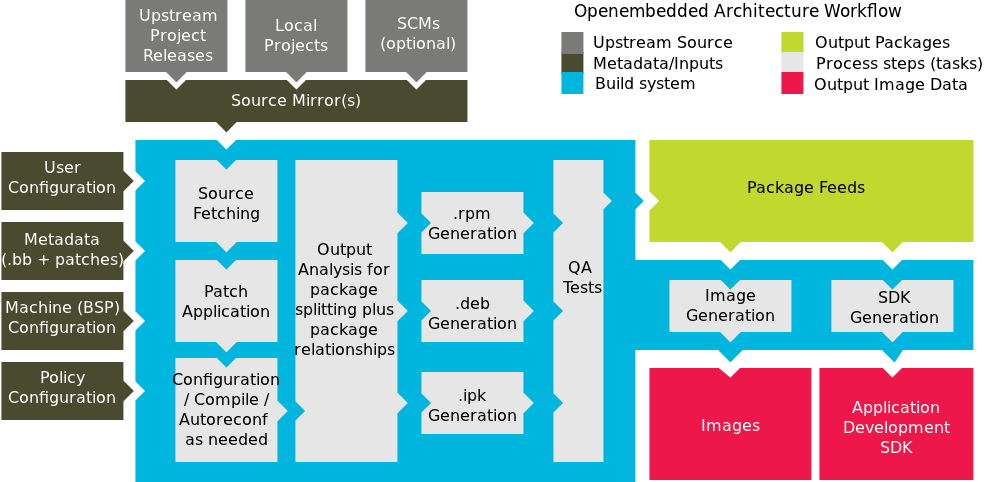
\includegraphics[width=180px]{assets/diagrams/yocto-environment.png}
      \caption{Source: \href{https://docs.yoctoproject.org}{https://docs.yoctoproject.org}\hspace{\textwidth}
      \it High-level diagram representing how builds work using The Yocto Project}
    \end{figure}
\end{frame}

\begin{frame}
  \frametitle{Custom Linux Image for the STM32MP1-DK2}
  \begin{minipage}{0.475\textwidth}
    \begin{block}{What is used in the deployed image?}
      \begin{itemize}
        \item ST's BSP (board support package) layer provides metadata 
          \begin{itemize}
            \small
            \item Hardware drivers
            \item Kernel Configurations
            \item Devicetree
          \end{itemize}
        \item Custom layer \DarkBoldP{meta-zf-project}
          \begin{itemize}
            \small
            \item \DarkBold{nginx} (webserver), \DarkBold{wpa\_supplicant} (Wi-Fi access client/
              IEEE 802.1X supplicant)
            \item recipes for custom applications (Web application, Server, Cortex-M4 Firmware)
            \item Kernel configurations and custom Devicetree
          \end{itemize}
      \end{itemize}
    \end{block}
  \end{minipage}
  \hfill
  \begin{minipage}{0.5\textwidth}
    \begin{figure}
      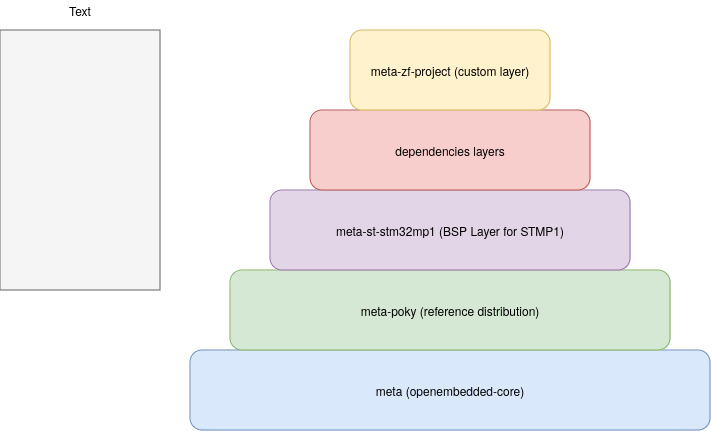
\includegraphics[width=1.125\textwidth]{assets/diagrams/layers.png}
      \caption{\it Layer Model representation of this project for deploying onto a 
      STM32MP1-DK2}
    \end{figure}
  \end{minipage}
\end{frame}

%==============================================================================
% DESIGN AND IMPLEMENTATION SECTION: IPC with OpenAMP
%==============================================================================
\subsection{Inter-Processor Communication}
\begin{frame}
  \frametitle{Inter-Process Communication on a Heterogenous Architecture}
  With a heterogenous architecture (ARM Cortex-A7 and ARM Cortex-M4) how can information be shared?\\
  {\em \scriptsize Hetergenous multiprocessor SoCs cannot directly communicate }
  \break
  \begin{minipage}{0.465\textwidth}
    \begin{block}{OpenAMP (Asymmetric Multi-Processing) Project}
      \footnotesize
      \begin{itemize}
        \item Software framework that places standard protocol for shared memory
        \item Implemented on top of \DarkBoldP{virtio} framework
        \item STM provides \DarkBoldP{virt\_uart} driver for recieving/transmitting messages
          over \DarkBoldP{RPMsg protocol}
        \item STMP1 layer automatically enables the \DarkBoldP{RPMSG tty driver} kernel module
          \begin{itemize}
              \tiny
            \item creates file in Linux filesystem: \DarkBoldP{/dev/ttyRPMSG<X>}
            \item can read and write to like a normal file
          \end{itemize}
        \item \DarkBoldP{remoteproc} framework allows dynamic and remote loading of Cortex-M4 firmware
        \item \LightBold{Resource Table} defined in firmware opens a trace in\\
          {\scriptsize\DarkBoldP{/sys/kernel/debug/remoteproc/remoteproc0/trace0}}
          \begin{itemize}
              \tiny
            \item Used for logging measured data in CSV format
          \end{itemize}
      \end{itemize}
    \end{block}
  \end{minipage}
  \hfill
  \begin{minipage}{0.465\textwidth}
    \begin{figure}
      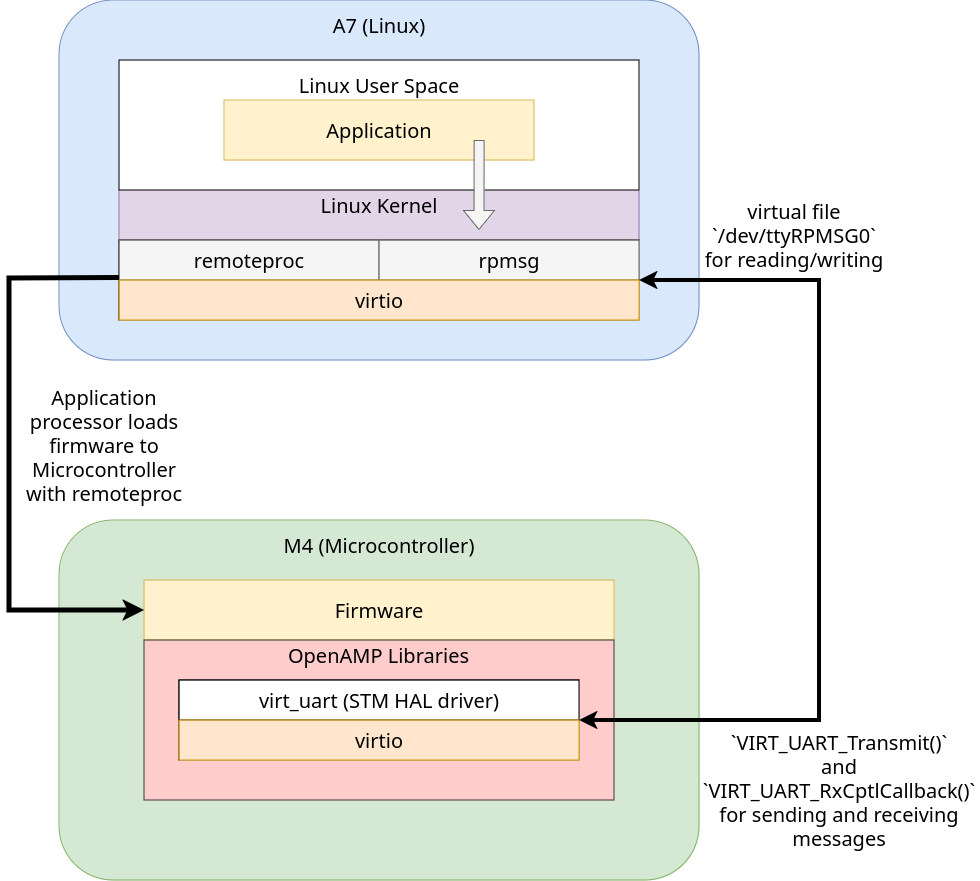
\includegraphics[width=\textwidth]{assets/diagrams/ipc.drawio.png}
      \caption{Inter-processor communication between Cortex-A7 (Linux) and Cortex-M4 (Microcontroller)}
    \end{figure}
  \end{minipage}
\end{frame}

%==============================================================================
% DESIGN AND IMPLEMENTATION SECTION: Rust
%==============================================================================
\subsection{Rust}
\begin{frame}
  \frametitle{Rust}
  \begin{minipage}{0.75\textwidth}
    The Rust programming language was used to write both major \\ 
    applications (web-based application and web server) for 2 main \\ reasons.
  \end{minipage}
  \hfill
  \begin{minipage}{0.20\textwidth}
    \begin{figure}
      
\includegraphics[width=\textwidth]{assets/misc/rewrite-it-in-rust.jpg}
      \caption{\it Ferris, universally accepted mascot of the Rust Programming language}
    \end{figure}

  \end{minipage}
  \hfill
  \vspace{-8px}
  \begin{block}{Memory Safety and Performance}
    \begin{itemize}
      \item A set of rules called \DarkBold{Ownership} enforced by compiler to prevent memory leaks
      \item \DarkBold{Borrow checker} within the compiler prevents programs unsafe programs from compiling*
      \item Nearly as or just as performant as C with \DarkBold{Zero Cost Abstractions}
      \item Advocated by/used by several United States goverment agencies:
        \begin{itemize}
          \item \LightBold{National Security Agency (NSA)} and 
            \LightBold{Cybersecurity and Infrastructure Security Agency (CISA)} in a paper:
            \ul{The Case for Memory Safe Roadmaps:
            Why Both C-Suite Executives and Technical Experts
            Need to Take Memory Safe Coding Seriously}
          \item \LightBold{Defense Advance Research Projects Agency} with their \LightBold{TRACTR: Translate All C To Rust} program
          \item \LightBold{The White House} in a Press Release: \ul{Future Software Should be Memory Safe}
        \end{itemize}
    \end{itemize}
  \end{block}
\end{frame}

%==============================================================================
% DESIGN AND IMPLEMENTATION SECTION: Web-Assembly Application
%==============================================================================

\begin{frame}
  \frametitle{Web-Application for User Interface}
  \begin{minipage}{0.5\textwidth}
    \begin{block}{Web Application in WebAssembly (WASM)}
      \begin{itemize}
        \item WASM is a compiled, binary format executable 
        \item Much faster than traditional Javascript programs
        \item Using the Yew framework, written in Rust
      \end{itemize}
    \end{block}
    \begin{block}{Web application Features}
      \begin{itemize}
        \item Shows if application is connected to associated server
        \item Selection of different devices
        \item Shows progress and state of test
        \item Allows download to results in a CSV
      \end{itemize}
    \end{block}
  \end{minipage}
  \hfill
  \begin{minipage}{0.4\textwidth}
    \begin{figure}
      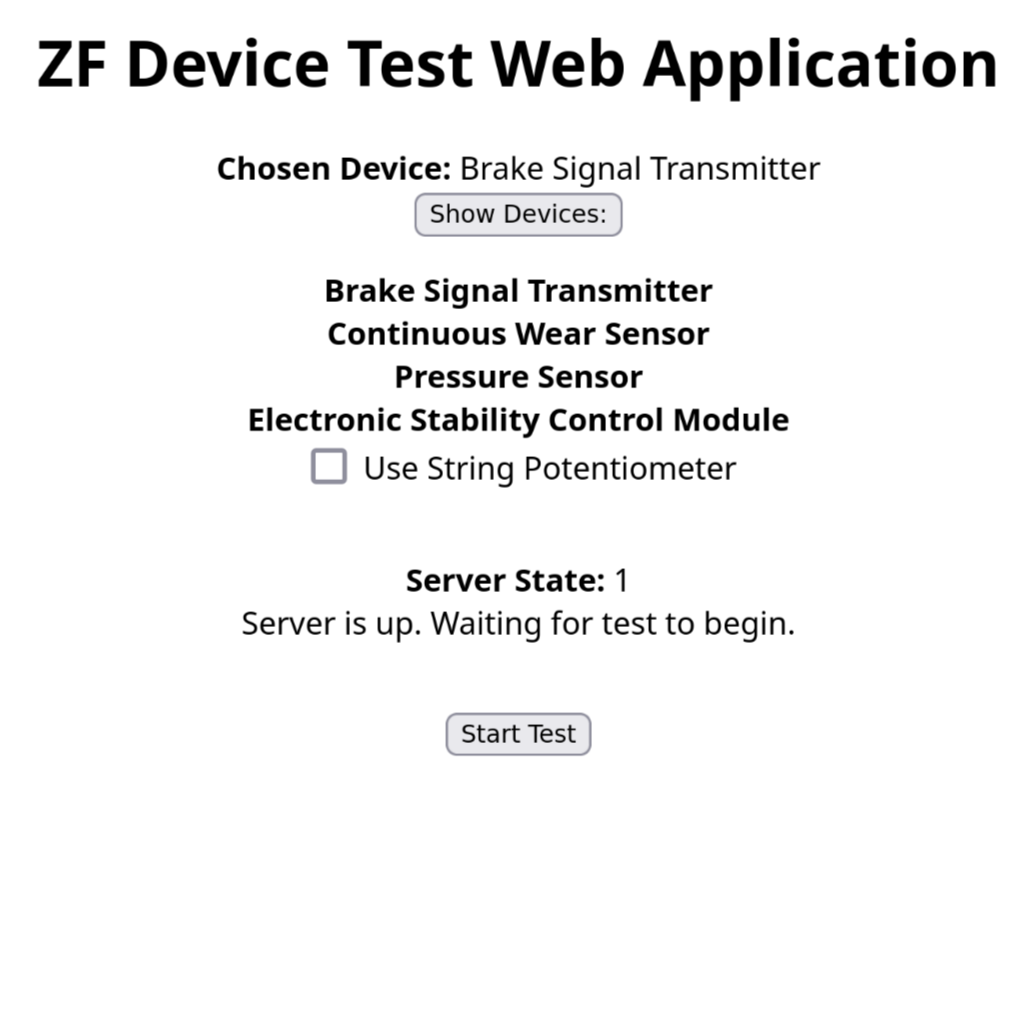
\includegraphics[width=\textwidth]{assets/misc/webapp.png}
      \caption{\it Web application with dropdown selection of different devices}
    \end{figure}
  \end{minipage}
\end{frame}

\begin{frame}
  \frametitle{Custom API Web Server}
  \begin{minipage}{0.5\textwidth}
    \begin{block}{Web Server features}
      \begin{itemize}
        \item Handles \DarkBoldP{HTTP requests} from web application
        \item Dynamically loads M4 Firmware for selected device with \DarkBoldP{remoteproc}
        \item Polls for results by reading and writing to \DarkBoldP{/dev/ttyRPMSG0} 
        \item Saves information from \DarkBoldP{/sys/kernel/debug/remoteproc/remoteproc0/trace0} as CSV for download
      \end{itemize}
    \end{block}
  \end{minipage}
  \hfill
  \begin{minipage}{0.4\textwidth}
    \begin{figure}
      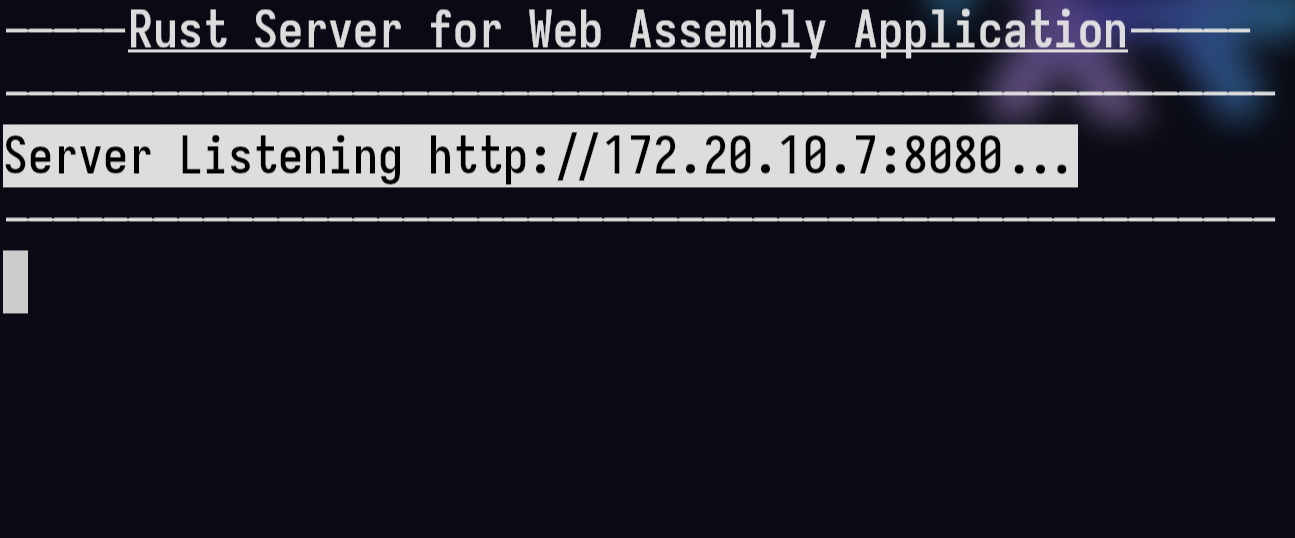
\includegraphics[width=\textwidth]{assets/misc/server1.png}
      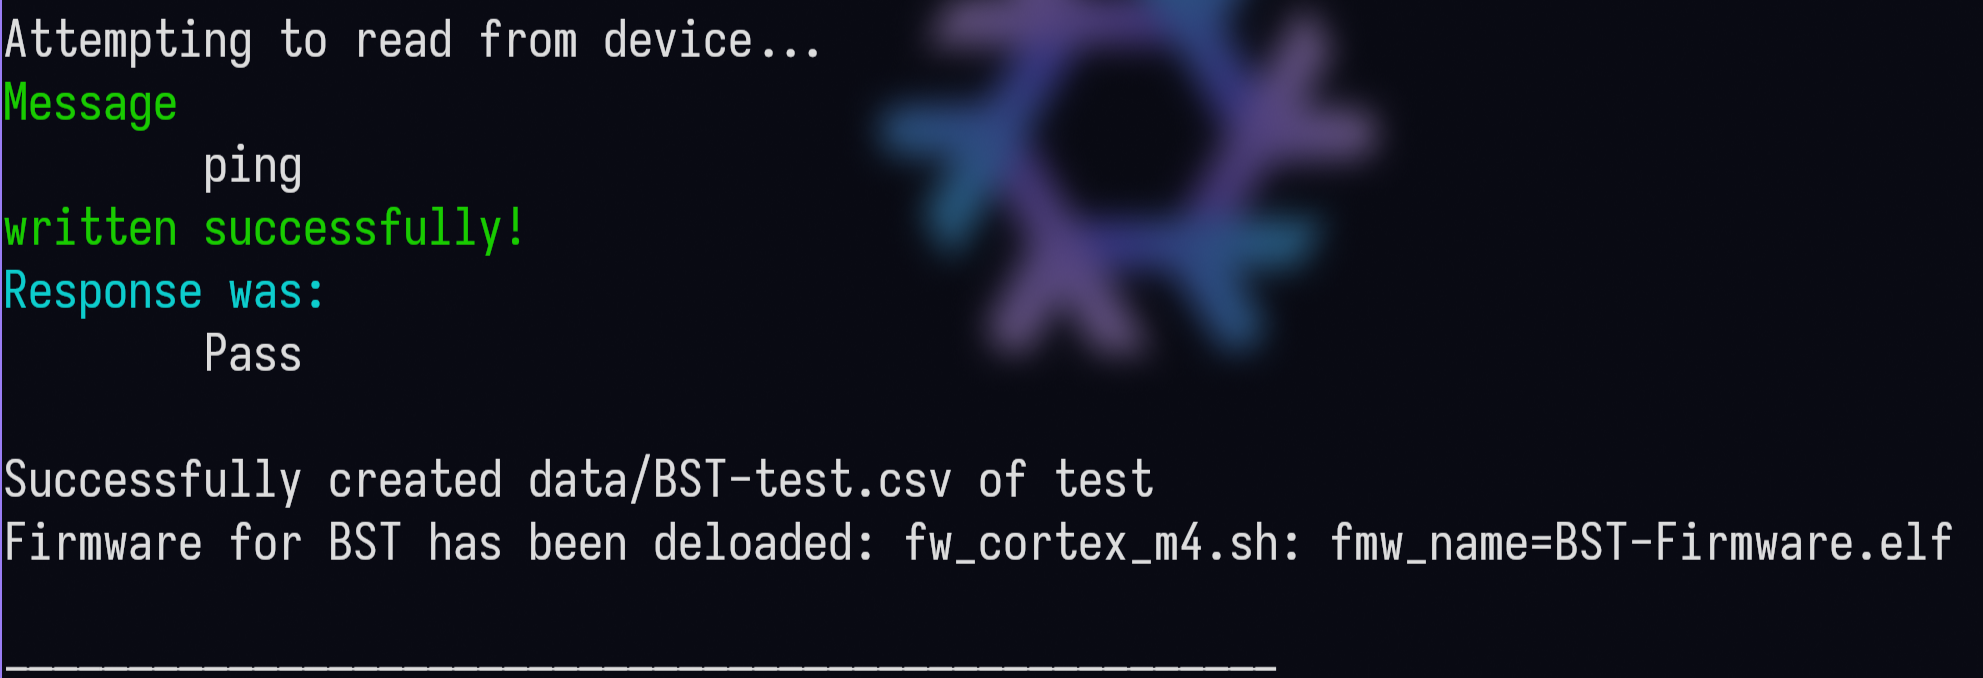
\includegraphics[width=\textwidth]{assets/misc/server2.png}
      \caption{\it Console logging of server application}
    \end{figure}
  \end{minipage}
\end{frame}

\begin{frame}
  \frametitle{Software Architecture}
  \begin{figure}
    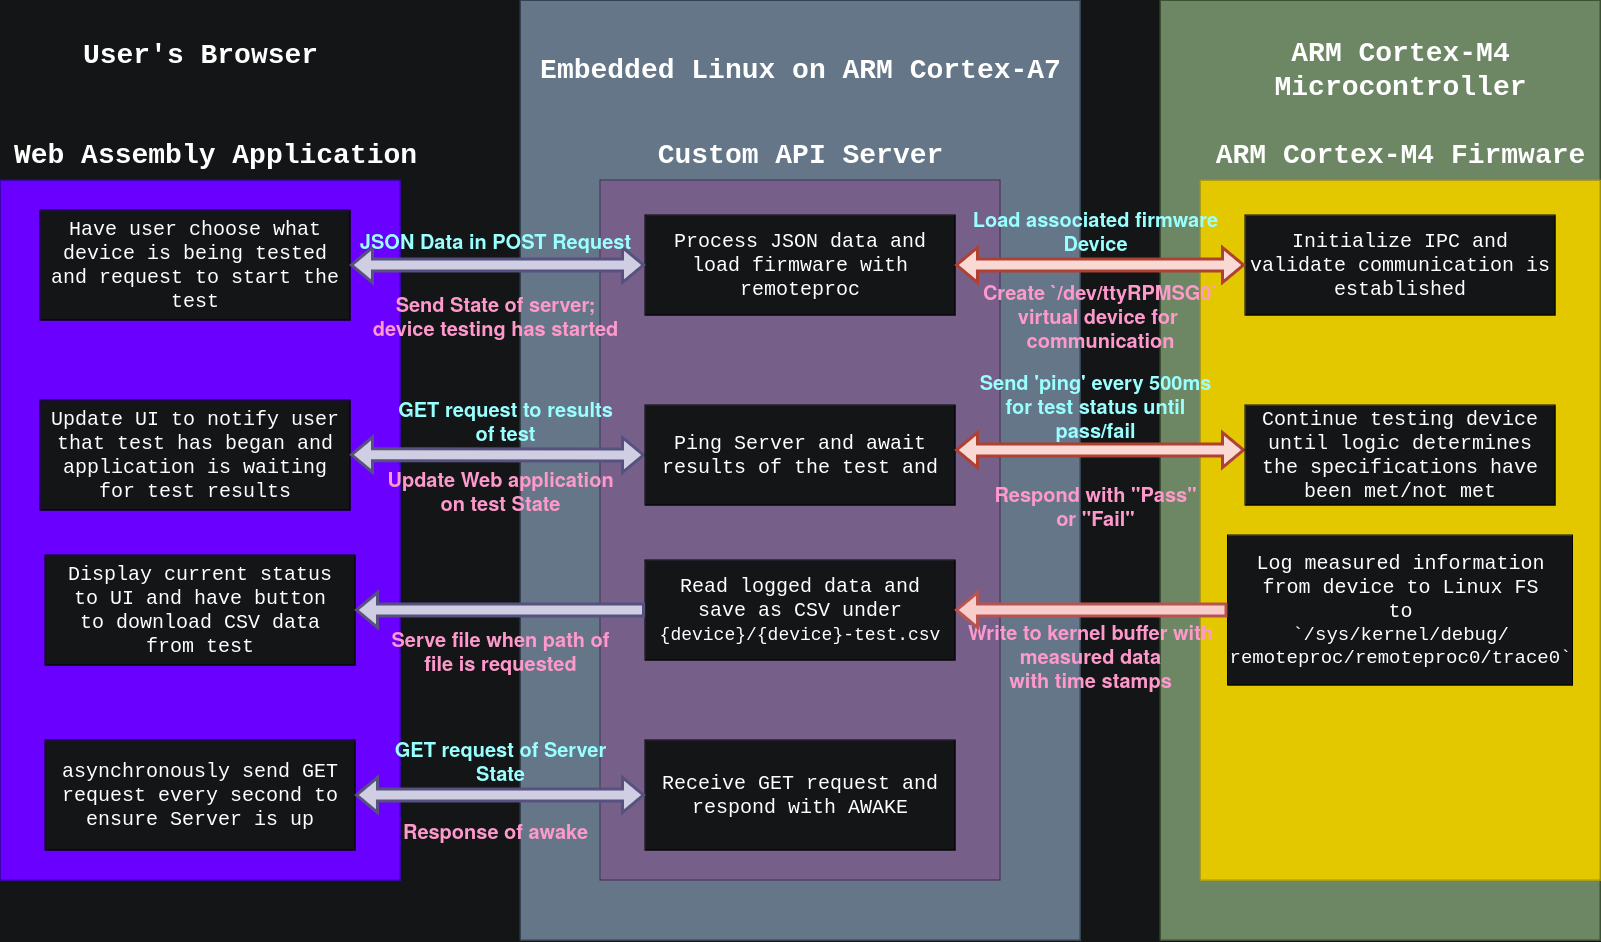
\includegraphics[width=\textwidth]{assets/diagrams/software_stack.drawio.png}
  \end{figure}
\end{frame}

\section{Verifcation}
\begin{frame}
  \begin{block}{Link to video demonstration}
    \href{https://dylxndy.xyz/senior-design-presentation/verification}
    {\color{lime}{\ul{https://dylxndy.xyz/senior-design-presentation/verification}}}
  \end{block}
\end{frame}

\section{Challenges}
\begin{frame}
  \frametitle{Challenges}
  \begin{itemize}
    \item System Clock configuration with Devicetree
  \end{itemize}
\end{frame}

\section{Future Work}
\begin{frame}
  \frametitle{Future Work}
  \begin{itemize}
    \item Finish CAN implementation for ESCM
      \begin{itemize}
        \item USB to CAN used currently
        \item enabled \DarkBoldP{CAN\_GS\_USB} module in Linux Kernel
      \end{itemize}
    \item Improve Web application apperance
  \end{itemize}

\end{frame}

\section{Closing}
\begin{frame}
  \frametitle{Special Thanks}
  \begin{itemize}
    \item Dr. Grantner (faculty advisor)
    \item David Florida (lab technician)
    \item Patrick McNally (Head of Engineering at ZF Group - Auburn Hills, MI)
    \item Davis Roman (Senior Staff Software Engineer at Rivian - Palo Alto, CA)
  \end{itemize}
\end{frame}

\begin{frame}
  \frametitle{Thank you}
  Any Questions?
  \begin{block}{Project Sources}
    \begin{itemize}
      \item \DarkBoldP{Custom Yocto Project Layer:}
        \begin{itemize}
          \item \url{https://github.com/DMGDy/meta-zf-project}
        \end{itemize}
      \item \DarkBoldP{Custom Web Server in Rust} 
        \begin{itemize}
          \item \url{https://github.com/DMGDy/zf-webserver-app}
        \end{itemize}
      \item \DarkBoldP{Web Application in WASM}
        \begin{itemize}
          \item  \url{https://github.com/DMGDy/zf-yew-app}
        \end{itemize}
      \item \DarkBoldP{Microcontroller Firmware}
        \begin{itemize}
          \item \url{https://github.com/danb127/Brake-System-Tester}
        \end{itemize}
      \item \DarkBoldP{This Presentation}
        \begin{itemize}
          \item \url{https://github.com/DMGDy/ECE4820-Presentation}
        \end{itemize}
    \end{itemize}
  \end{block}
\end{frame}



\end{document}
